\documentclass[11pt,a4paper]{article}
\usepackage[utf8]{inputenc}
\usepackage[T1]{fontenc}
\usepackage[brazil]{babel}
\usepackage{amsmath,amssymb}
\usepackage{graphicx}
\usepackage{geometry}
\usepackage{enumitem}
\usepackage{array,booktabs,tabularx}
\usepackage{xcolor}
\usepackage{fancyhdr}
\usepackage{microtype}
\usepackage[most]{tcolorbox}
\usepackage{helvet}
\usepackage{caption}
\usepackage{float}
\usepackage{hyperref}
\renewcommand{\familydefault}{\sfdefault}

\geometry{top=20mm,bottom=20mm,left=22mm,right=22mm}
\definecolor{unirblue}{HTML}{0B4EA2}
\definecolor{ink}{HTML}{172033}
\definecolor{muted}{HTML}{667085}
\definecolor{soft}{HTML}{F5F7FA}
\definecolor{line}{HTML}{D7DCE2}
\definecolor{guide}{HTML}{EEF4FB}

\hypersetup{colorlinks=true,linkcolor=unirblue,urlcolor=unirblue,citecolor=unirblue}
\setlength{\parindent}{0pt}
\setlength{\parskip}{5pt}
\setlist[itemize]{leftmargin=5mm,itemsep=2pt,topsep=2pt}
\setlist[enumerate]{leftmargin=6mm,itemsep=2pt,topsep=2pt}
\captionsetup{font=small,labelfont=bf}

\pagestyle{fancy}
\fancyhf{}
\renewcommand{\headrulewidth}{0pt}
\cfoot{\color{muted}\footnotesize UNIR · Processamento de Imagens · Relatório da Avaliação \hfill \thepage}

\newcommand{\sectiontitle}[1]{%
  \vspace{5pt}{\Large\bfseries\color{ink}#1}\par
  \vspace{1mm}{\color{unirblue}\rule{\textwidth}{0.8pt}}\vspace{2mm}}
\newcommand{\subsectiontitle}[1]{\vspace{4pt}{\large\bfseries\color{ink}#1}\par\vspace{1mm}}
\newcommand{\placeholder}[1]{\textcolor{muted}{\textit{#1}}}

\newtcolorbox{orientacao}{
  colback=guide,
  colframe=unirblue!25,
  leftrule=2pt,rightrule=0pt,toprule=0pt,bottomrule=0pt,
  arc=0mm,boxsep=1.5mm,left=2mm,right=2mm,top=1.5mm,bottom=1.5mm,
  fontupper=\small\color{ink}
}

\newtcolorbox{campo}{
  colback=soft,colframe=line,boxrule=.4pt,arc=1mm,
  left=2mm,right=2mm,top=2mm,bottom=2mm
}

% ------------------------------------------------------------
% Imagens: logo, diagrama e captura da interface ficam em imagens/ (nesta
% pasta); os resultados são gerados por ./build/cinzel_relatorio em
% ../../imagens/saida/ (pasta imagens/ da raiz do projeto)
% ------------------------------------------------------------
\graphicspath{{imagens/}{../../imagens/saida/}}

% \celula{largura relativa}{arquivo}{legenda curta}
\newcommand{\celula}[3]{%
  \begin{minipage}[t]{#1\textwidth}\centering
    \includegraphics[width=\linewidth]{#2}\par\vspace{0.5mm}
    {\scriptsize #3}
  \end{minipage}}

\begin{document}

% ============================================================
% CAPA
% ============================================================
\begin{titlepage}
\thispagestyle{empty}

\begin{center}
  
\includegraphics[width=4.8cm]{unir_logo.png}
\end{center}

\vspace{8mm}

\begin{center}
{\small\bfseries\color{muted} FUNDAÇÃO UNIVERSIDADE FEDERAL DE RONDÔNIA - UNIR}\\[2mm]
{\small\color{muted} Faculdade de Engenharia, Tecnologia e Inovação - FAETI}\\
{\small\color{muted} Bacharelado em Ciência da Computação}
\end{center}

\vfill

\begin{center}
{\small\bfseries\color{unirblue} PROCESSAMENTO DE IMAGENS}\\[5mm]
{\Huge\bfseries\color{ink} Relatório da Primeira Avaliação}\\[3mm]
{\large\color{muted} Cinzel: Sistema de Processamento de Imagens em Escala de Cinza}\\[12mm]

{\Large\bfseries\color{ink} João Henrique Vieira do Carmo}\\[2mm]
{\small\color{muted} Matrícula: 20231009063}
\end{center}

\vfill

\begin{center}
{\small\color{muted} Professor: Lucas Marques da Cunha}\\[1mm]
{\small\color{muted} Porto Velho - RO}\\
{\small\color{muted} 2026}
\end{center}

\end{titlepage}

% ============================================================
% FOLHA DE IDENTIFICAÇÃO
% ============================================================
\sectiontitle{Identificação do trabalho}

\begin{campo}
\begin{tabularx}{\textwidth}{>{\bfseries}p{37mm}X}
Aluno(a): & \placeholder{João Henrique Vieira do Carmo}\\[2mm]
Matrícula: & \placeholder{20231009063}\\[2mm]
Disciplina: & Processamento de Imagens\\[2mm]
Professor: & Lucas Marques da Cunha\\[2mm]
Título do sistema: & Cinzel: Sistema de Processamento de Imagens em Escala de Cinza\\[2mm]
Linguagem/ambiente: & C++17 / aplicação desktop (Linux), interface com Dear ImGui\\[2mm]
Repositório: & \placeholder{https://github.com/Tatmiki/cinzel}\\
\end{tabularx}
\end{campo}

\vspace{3mm}
\tableofcontents
\newpage

% ============================================================
% 1 INTRODUÇÃO
% ============================================================
\section{Introdução}

Uma imagem digital é uma representação discreta de uma cena: uma grade de elementos
(\textit{pixels}) em que cada posição armazena uma intensidade. O processamento digital de
imagens reúne as técnicas que transformam essa grade para realçar informações, reduzir
degradações ou extrair estruturas de interesse, servindo de base para aplicações como
diagnóstico médico, sensoriamento remoto, inspeção industrial e visão computacional
\cite{gonzalez}.

Boa parte dessas técnicas é construída sobre um pequeno conjunto de operações fundamentais.
As \textbf{transformações de intensidade} alteram o valor de cada pixel isoladamente e
permitem corrigir imagens escuras, claras demais ou com pouco contraste. O \textbf{histograma}
descreve a distribuição dos níveis de cinza e orienta transformações globais de contraste,
como a expansão e a equalização. As operações \textbf{baseadas em vizinhança}, formalizadas
pela convolução, combinam cada pixel com os seus vizinhos para suavizar ruído, detectar
bordas ou aguçar detalhes.

Compreender essas operações exige mais do que usá-las prontas: cada uma envolve decisões de
implementação que afetam diretamente o resultado, como o tratamento dos pixels próximos à
borda da imagem, a conversão de valores que saem da faixa de 8 bits, a orientação das
máscaras e a escolha de parâmetros. Por isso, nesta avaliação todos os algoritmos foram
implementados integralmente, sem bibliotecas de processamento.

Este relatório documenta o \textbf{Cinzel}, um sistema desktop escrito em C++17 para
processamento de imagens em escala de cinza de 8 bits por pixel. O sistema implementa as
operações da Unidade 01 da disciplina, oferece uma interface gráfica para aplicá-las com
parâmetros ajustáveis e visualizar respostas intermediárias, e inclui um conjunto de testes
automatizados e um gerador das imagens de resultado apresentadas neste documento.

\subsection{Objetivos}

\textbf{Objetivo geral.} Desenvolver um sistema de processamento de imagens em escala de
cinza de 8 bits que implemente, sem bibliotecas de processamento, as operações fundamentais
da Unidade 01, permitindo aplicar, parametrizar e analisar cada uma delas.

\textbf{Objetivos específicos.}
\begin{itemize}
  \item Implementar operações algébricas (dissolve cruzado uniforme e não uniforme) e
        transformações de intensidade (negativo, alargamento de contraste, limiarização,
        potência e logaritmo).
  \item Implementar a expansão e a equalização de histograma e o controle de contraste
        adaptativo com constante $c$ e vizinhança $n \times n$ parametrizáveis.
  \item Implementar uma convolução genérica $g = f * h + \text{offset}$, com máscara
        $n \times m$, tratamento explícito das bordas e dos valores fora de $[0, 255]$.
  \item Implementar os filtros da média e da mediana com vizinhança parametrizável.
  \item Implementar os detectores de bordas de Roberts, Sobel, Kirsch e Laplaciano,
        exibindo $G_x$, $G_y$, a magnitude do gradiente e as respostas de cada máscara.
  \item Implementar o aguçamento pelo Laplaciano e a técnica \textit{high boost}, exibindo
        separadamente a resposta do operador e a imagem combinada.
  \item Executar e interpretar os testes obrigatórios de convolução (aguçamento, relevo e
        detecção de bordas).
\end{itemize}

% ============================================================
% 2 FUNDAMENTAÇÃO
% ============================================================
\section{Fundamentação teórica}

\subsection{Representação de imagens digitais e vizinhança}

Uma imagem em escala de cinza é modelada como uma função $f(x, y)$, em que $(x, y)$ são as
coordenadas espaciais (coluna e linha) e $f(x, y)$ é a intensidade no ponto. Em uma imagem
digital, as coordenadas são inteiras e as intensidades são quantizadas. Com 8 bits por pixel
há $L = 2^8 = 256$ níveis possíveis:
\begin{equation}
  f : \{0, \dots, M-1\} \times \{0, \dots, N-1\} \to \{0, 1, \dots, 255\},
\end{equation}
em que $M$ e $N$ são a largura e a altura, $0$ representa o preto e $255$ o branco
\cite{gonzalez}.

A \textbf{vizinhança} de um pixel é o conjunto de pixels próximos a ele. As mais comuns são
a vizinhança-4 (os quatro vizinhos horizontais e verticais), a vizinhança-8 (inclui as
diagonais) e, de forma geral, uma janela $n \times m$ centrada no pixel. Operações de
vizinhança precisam definir o que fazer quando a janela ultrapassa os limites da imagem. Para
isso define-se uma imagem estendida $\tilde f$, igual a $f$ dentro da imagem e definida por
uma estratégia fora dela:
\begin{itemize}
  \item \textbf{Zero:} $\tilde f(x, y) = 0$ fora da imagem, o que tende a escurecer a moldura.
  \item \textbf{Replicação:} usa o pixel da borda mais próximo,
        $\tilde f(x, y) = f(\mathrm{clamp}(x, 0, M-1),\, \mathrm{clamp}(y, 0, N-1))$.
  \item \textbf{Reflexão:} espelha a imagem na borda ($x = -1 \mapsto 1$,
        $x = M \mapsto M - 2$).
  \item \textbf{Circular:} trata a imagem como periódica ($x = -1 \mapsto M - 1$).
\end{itemize}

\subsection{Operações algébricas e transformações de intensidade}

\textbf{Dissolve cruzado.} Combina duas imagens $f_1$ e $f_2$ de mesmo tamanho por média
ponderada. No dissolve \textbf{uniforme}, o peso $t \in [0, 1]$ é o mesmo para todos os
pixels; variando $t$ de 0 a 1, a imagem passa gradualmente de $f_1$ para $f_2$. No
\textbf{não uniforme}, o peso varia com a posição, $t(x, y)$, permitindo transições
espaciais (por exemplo, uma rampa horizontal ou um padrão radial):
\begin{equation}
  g(x, y) = \big(1 - t(x,y)\big)\, f_1(x, y) + t(x,y)\, f_2(x, y).
\end{equation}

\textbf{Transformações de intensidade} são operações pontuais da forma $s = T(r)$, em que
$r$ é o nível de entrada e $s$ o de saída: o resultado em cada pixel depende apenas do valor
daquele pixel \cite{gonzalez}.

\begin{itemize}
  \item \textbf{Negativo:} $s = 255 - r$. Inverte a escala de cinza, realçando detalhes
        claros em regiões escuras extensas.
  \item \textbf{Limiarização:} $s = 255$ se $r \geq T$ e $s = 0$ caso contrário. Produz uma
        imagem binária, separando objetos do fundo segundo o limiar $T$.
  \item \textbf{Alargamento de contraste:} função linear por partes definida pelos pontos
        $(r_1, s_1)$ e $(r_2, s_2)$:
\begin{equation}
  s = \begin{cases}
    \dfrac{s_1}{r_1}\, r, & r < r_1,\\[2mm]
    s_1 + \dfrac{s_2 - s_1}{r_2 - r_1}\,(r - r_1), & r_1 \le r \le r_2,\\[2mm]
    s_2 + \dfrac{255 - s_2}{255 - r_2}\,(r - r_2), & r > r_2.
  \end{cases}
\end{equation}
        A inclinação do segmento central, $(s_2 - s_1)/(r_2 - r_1)$, é maior que 1 quando
        se deseja ampliar o contraste da faixa $[r_1, r_2]$.
  \item \textbf{Potência (gamma):} com $r$ normalizado para $[0, 1]$,
\begin{equation}
  s = 255 \cdot c \left(\frac{r}{255}\right)^{\gamma}.
\end{equation}
        Para $\gamma < 1$ a curva fica acima da identidade e expande os tons escuros
        (clareia); para $\gamma = 1$ (e $c = 1$) é a identidade; para $\gamma > 1$ a curva
        fica abaixo da identidade e expande os tons claros (escurece).
  \item \textbf{Logaritmo:} $s = c \log(1 + r)$. Expande fortemente os níveis baixos e
        comprime os altos. Com $c = 255/\ln 256 \approx 45{,}99$, o nível 255 é mapeado
        em 255.
\end{itemize}

\subsection{Histograma}

O histograma de uma imagem conta quantos pixels possuem cada nível de cinza. Normalizado
pelo total $N$ de pixels, ele estima a probabilidade de ocorrência de cada nível:
\begin{equation}
  h(k) = \#\{(x, y) : f(x, y) = k\}, \qquad p(k) = \frac{h(k)}{N}.
\end{equation}
Imagens escuras concentram o histograma à esquerda, imagens claras à direita e imagens de
baixo contraste em uma faixa estreita.

A \textbf{expansão} de histograma é uma transformação linear que leva a faixa ocupada
$[r_{\min}, r_{\max}]$ para toda a faixa $[0, 255]$:
\begin{equation}
  s = \frac{r - r_{\min}}{r_{\max} - r_{\min}} \cdot 255.
\end{equation}
Ela não altera a forma do histograma, apenas o ``estica''. Se a imagem já possui pixels
próximos de 0 e de 255, o efeito é quase nulo.

A \textbf{equalização} usa a distribuição acumulada (CDF) como transformação, buscando um
histograma aproximadamente uniforme \cite{gonzalez}:
\begin{equation}
  s_k = \mathrm{round}\!\left(255 \sum_{j=0}^{k} p(j)\right).
\end{equation}
É uma transformação não linear que depende do conteúdo: níveis muito frequentes recebem
uma faixa maior da escala de saída e níveis raros são agrupados. Como a imagem é discreta,
o histograma resultante não é perfeitamente plano, e níveis distintos podem ser fundidos.

\subsection{Filtragem espacial e convolução}

Operações baseadas em vizinhança calculam cada pixel de saída a partir de uma janela de
pixels de entrada. A forma linear dessas operações é a \textbf{convolução} com uma máscara
$h$ de dimensão $n \times m$. Indexando a máscara pelo deslocamento $(s, t)$ em relação ao
seu centro, com $a = \lfloor (n-1)/2 \rfloor$ e $b = \lfloor (m-1)/2 \rfloor$:
\begin{equation}
  (h * f)(x, y) = \sum_{s} \sum_{t} h(s, t)\, \tilde f(x - t,\, y - s).
\end{equation}
A \textbf{correlação} tem a mesma forma, mas com $\tilde f(x + t, y + s)$; a convolução
equivale, portanto, a rotacionar a máscara em $180^\circ$ antes de aplicar a correlação.
Para máscaras simétricas as duas operações coincidem; para máscaras assimétricas (relevo,
detectores direcionais) o resultado muda de sentido \cite{gonzalez}.

Em regiões de intensidade constante $v$, a resposta da máscara é $v \sum h(s,t)$. A soma dos
coeficientes indica, portanto, o comportamento global do filtro: soma 1 preserva o brilho
médio (suavização normalizada, aguçamento), soma 0 anula regiões uniformes e mantém apenas as
variações (detecção de bordas, relevo), soma maior que 1 clareia e soma negativa inverte.
Como as máscaras podem ter coeficientes negativos e somas diferentes de 1, a convolução pode
produzir valores negativos ou maiores que 255, que precisam de tratamento antes da conversão
para 8 bits.

O \textbf{filtro da média} substitui cada pixel pela média aritmética da vizinhança
$n \times n$, o que equivale à convolução com uma máscara de coeficientes $1/n^2$. É um
filtro \textbf{linear}: reduz ruído aleatório, mas também borra bordas e espalha ruído
impulsivo, já que um único valor extremo altera a média de toda a janela.

O \textbf{filtro da mediana} ordena os valores da vizinhança e escolhe o valor central. É
\textbf{não linear} (a mediana de uma soma não é a soma das medianas) e, portanto, não pode
ser expresso como convolução. É especialmente eficaz contra ruído impulsivo
(sal-e-pimenta), pois valores extremos isolados vão para as pontas da lista ordenada e são
descartados, preservando melhor as bordas \cite{gonzalez,pedrini}.

\subsection{Detecção de bordas}

Bordas são regiões de variação brusca de intensidade e podem ser detectadas por derivadas.
Os operadores de \textbf{primeira derivada} estimam o gradiente
\begin{equation}
  \nabla f = \begin{bmatrix} G_x \\ G_y \end{bmatrix}
           = \begin{bmatrix} \partial f / \partial x \\ \partial f / \partial y \end{bmatrix},
  \qquad
  |\nabla f| = \sqrt{G_x^2 + G_y^2} \approx |G_x| + |G_y|,
\end{equation}
em que $G_x$ responde a variações horizontais (bordas verticais) e $G_y$ a variações
verticais (bordas horizontais). A magnitude combina as duas componentes em uma medida de
intensidade de borda independente da orientação.

\textbf{Roberts} usa duas máscaras $2 \times 2$ que estimam derivadas nas diagonais:
\begin{equation}
  G_x: \begin{bmatrix} 1 & 0 \\ 0 & -1 \end{bmatrix}, \qquad
  G_y: \begin{bmatrix} 0 & 1 \\ -1 & 0 \end{bmatrix}.
\end{equation}
Por usar apenas quatro pixels, é rápido e produz bordas finas, mas é muito sensível a ruído.

\textbf{Sobel} usa máscaras $3 \times 3$ que combinam a diferença em uma direção com uma
suavização na direção perpendicular (peso 2 na linha ou coluna central), o que o torna
menos sensível a ruído:
\begin{equation}
  G_x: \begin{bmatrix} -1 & 0 & 1 \\ -2 & 0 & 2 \\ -1 & 0 & 1 \end{bmatrix}, \qquad
  G_y: \begin{bmatrix} -1 & -2 & -1 \\ 0 & 0 & 0 \\ 1 & 2 & 1 \end{bmatrix}.
\end{equation}

\textbf{Kirsch} é um operador de bússola com oito máscaras $3 \times 3$, obtidas girando em
$45^\circ$ os coeficientes do anel externo da máscara base \cite{kirsch}:
\begin{equation}
  K_0 = \begin{bmatrix} 5 & 5 & 5 \\ -3 & 0 & -3 \\ -3 & -3 & -3 \end{bmatrix}, \quad
  K_1 = \begin{bmatrix} -3 & 5 & 5 \\ -3 & 0 & 5 \\ -3 & -3 & -3 \end{bmatrix}, \quad
  \dots, \quad
  K_7 = \begin{bmatrix} 5 & 5 & -3 \\ 5 & 0 & -3 \\ -3 & -3 & -3 \end{bmatrix}.
\end{equation}
Cada máscara responde mais fortemente a bordas em uma das oito orientações. Como uma borda
tem uma única orientação dominante em cada ponto, a resposta do operador é a maior entre as
oito, $g = \max_k (K_k * f)$, e a máscara vencedora indica a direção da borda. Todas as
máscaras somam zero, de modo que regiões uniformes produzem resposta nula.

O \textbf{Laplaciano} é um operador isotrópico de \textbf{segunda derivada}:
\begin{equation}
  \nabla^2 f = \frac{\partial^2 f}{\partial x^2} + \frac{\partial^2 f}{\partial y^2}
  \approx f(x{+}1,y) + f(x{-}1,y) + f(x,y{+}1) + f(x,y{-}1) - 4f(x,y),
\end{equation}
que corresponde à máscara de 4 vizinhos; a versão de 8 vizinhos inclui as diagonais
(centro $-8$):
\begin{equation}
  \begin{bmatrix} 0 & 1 & 0 \\ 1 & -4 & 1 \\ 0 & 1 & 0 \end{bmatrix}, \qquad
  \begin{bmatrix} 1 & 1 & 1 \\ 1 & -8 & 1 \\ 1 & 1 & 1 \end{bmatrix}.
\end{equation}
O Laplaciano produz uma resposta dupla (positiva de um lado da borda e negativa do outro,
cruzando o zero sobre ela), não fornece direção e é bastante sensível a ruído, pois
derivadas de segunda ordem amplificam variações finas.

\subsection{Aguçamento}

O aguçamento realça detalhes finos e transições, aproximando a percepção de nitidez.
Diferentemente da detecção de bordas, cujo resultado é apenas um mapa de variações (regiões
uniformes viram zero), o aguçamento preserva o conteúdo da imagem e adiciona a ele as
variações realçadas.

\textbf{Aguçamento pelo Laplaciano.} A resposta do Laplaciano é combinada com a imagem
original \cite{gonzalez}:
\begin{equation}
  g(x, y) = f(x, y) + c\, \nabla^2 f(x, y),
\end{equation}
com $c = -1$ quando o coeficiente central da máscara é negativo (como nas máscaras acima) e
$c = +1$ quando é positivo. A regra garante que um pixel mais claro que os vizinhos (que gera
Laplaciano negativo com centro negativo) fique ainda mais claro. A combinação com a
original é necessária porque o Laplaciano isolado elimina a informação de fundo. Com o
Laplaciano de 8 vizinhos e $c = -1$, as duas operações se reduzem a uma única máscara:
\begin{equation}
  g = f - \nabla^2 f \;\Longleftrightarrow\;
  h = \begin{bmatrix} -1 & -1 & -1 \\ -1 & 9 & -1 \\ -1 & -1 & -1 \end{bmatrix}.
\end{equation}

\textbf{\textit{Unsharp masking} e \textit{high boost}.} Subtrai-se da imagem uma versão
suavizada $\bar f$, obtendo uma máscara de nitidez que contém só os detalhes, e soma-se essa
máscara ponderada à original:
\begin{equation}
  g(x, y) = f(x, y) + k\,\big(f(x, y) - \bar f(x, y)\big).
\end{equation}
Com $k = 1$ tem-se o \textit{unsharp masking}; com $k > 1$, o \textit{high boost}, que
realça os detalhes com mais intensidade \cite{gonzalez}.

\subsection{Controle de contraste adaptativo}

Transformações globais aplicam a mesma função a toda a imagem e podem não realçar detalhes
em regiões de baixo contraste local. O controle de contraste adaptativo ajusta cada pixel
segundo as estatísticas da sua vizinhança $n \times n$ \cite{gonzalez}: a média local
$m(x,y)$ e o desvio padrão local $\sigma(x,y)$, com $N = n^2$ pixels na janela $W$:
\begin{equation}
  m(x, y) = \frac{1}{N} \sum_{(i,j) \in W} \tilde f(i, j), \qquad
  \sigma(x, y) = \sqrt{\frac{1}{N} \sum_{(i,j) \in W} \tilde f(i, j)^2 - m(x, y)^2}.
\end{equation}
A formulação adotada neste trabalho segue o método de ganho local de \cite{narendra}, que
amplifica o desvio de cada pixel em relação à média local por um ganho inversamente
proporcional ao desvio padrão local. Na proposta original o ganho é $\alpha M / \sigma$, em que
$M$ é a média global da imagem; aqui o numerador $\alpha M$ é substituído por uma única
constante $c$:
\begin{equation}
  g(x, y) = m(x, y) + \frac{c}{\sigma(x, y)}\,\big(f(x, y) - m(x, y)\big).
\end{equation}
Em regiões de pouco contraste ($\sigma$ pequeno), o ganho $c/\sigma$ é grande e os detalhes
são realçados; em regiões já contrastadas ($\sigma$ grande), o ganho é pequeno. A constante
$c$ controla a intensidade do realce, e a dimensão $n$ define a escala do que é considerado
``local''. Em regiões perfeitamente uniformes ($\sigma = 0$) o pixel é mantido.

% ============================================================
% 3 MATERIAIS E MÉTODOS
% ============================================================
\section{Materiais e métodos}

\subsection{Ambiente de desenvolvimento}

O sistema foi desenvolvido em \textbf{C++17}, compilado com \textbf{g++ 13.3} e organizado com
\textbf{CMake}, no sistema operacional \textbf{Ubuntu 24.04}, utilizando o editor
\textbf{Visual Studio Code}. A Tabela~\ref{tab:bibliotecas} lista as bibliotecas usadas. Todas
se limitam a leitura, escrita, exibição de imagens e construção da interface, como permitido
pela especificação; nenhuma delas executa os algoritmos avaliados, que foram implementados
integralmente no módulo \texttt{src/core}, usando apenas a biblioteca padrão do C++.

\begin{table}[H]
\centering
\small
\begin{tabularx}{\textwidth}{lX}
\toprule
\textbf{Biblioteca} & \textbf{Uso no sistema} \\
\midrule
stb\_image / stb\_image\_write & Leitura de PNG, JPG e BMP e escrita de PNG (arquivos de cabeçalho único). \\
libtiff 4.5 & Leitura de arquivos TIFF, formato da maioria das imagens de teste. \\
Dear ImGui 1.91 & Construção da interface gráfica (botões, controles deslizantes, exibição de imagens e histogramas). \\
GLFW 3.3 e OpenGL 3.3 & Criação da janela, captura de eventos e desenho das texturas na tela. \\
\bottomrule
\end{tabularx}
\caption{Bibliotecas externas e sua finalidade.}
\label{tab:bibliotecas}
\end{table}

Imagens coloridas são convertidas para cinza na leitura, com os pesos
$(77R + 150G + 29B)/256$, os mesmos utilizados pela stb\_image. A partir desse ponto o sistema
trabalha exclusivamente com uma intensidade de 8 bits por pixel.

\subsection{Arquitetura e organização do sistema}

O código foi dividido em três partes; a arquitetura da aplicação principal está na Figura~\ref{fig:arquitetura}:
\begin{itemize}
  \item \textbf{Núcleo} (\texttt{src/core}): todos os algoritmos, sem nenhuma dependência de
        interface. É compilado como uma biblioteca estática reutilizada pelos demais
        executáveis.
  \item \textbf{Interface} (\texttt{src/gui}, executável \texttt{cinzel}): apenas chama as
        funções do núcleo e exibe os resultados.
  \item \textbf{Testes} (\texttt{src/testes}): o executável \texttt{cinzel\_testes} verifica os
        algoritmos em matrizes pequenas com valores calculados à mão, e o executável
        \texttt{cinzel\_relatorio} gera em lote todas as imagens deste relatório.
\end{itemize}

A Tabela~\ref{tab:modulos} descreve os módulos do núcleo.

\begin{table}[H]
\centering
\small
\begin{tabularx}{\textwidth}{lX}
\toprule
\textbf{Módulo} & \textbf{Responsabilidade} \\
\midrule
\texttt{imagem} & Tipos \texttt{Imagem} e \texttt{ImagemF}, conversão entre eles e leitura/escrita de arquivos. \\
\texttt{bordas\_pixel} & Função \texttt{pixelComBorda}, único ponto de acesso a pixels fora da imagem. \\
\texttt{mascaras} & Tipo \texttt{Mascara} e todas as máscaras usadas (Roberts, Sobel, Kirsch, Laplaciano, testes). \\
\texttt{convolucao} & Convolução genérica $g = f * h + \text{offset}$. \\
\texttt{pontuais} & Negativo, limiarização, alargamento de contraste, potência e logaritmo. \\
\texttt{algebricas} & Dissolve cruzado uniforme e não uniforme. \\
\texttt{histograma} & Cálculo do histograma, expansão e equalização. \\
\texttt{filtros} & Filtros da média e da mediana. \\
\texttt{adaptativo} & Controle de contraste adaptativo. \\
\texttt{deteccao} & Operadores de Roberts, Sobel, Kirsch e Laplaciano. \\
\texttt{agucamento} & Aguçamento pelo Laplaciano e \textit{high boost}. \\
\bottomrule
\end{tabularx}
\caption{Módulos do núcleo de processamento.}
\label{tab:modulos}
\end{table}

As principais estruturas de dados são:
\begin{itemize}
  \item \texttt{Imagem}: largura, altura e um vetor de bytes (\texttt{uint8\_t}) em ordem de
        linhas, de modo que o pixel $(x, y)$ está no índice $y \cdot M + x$. É o tipo lido,
        exibido e salvo.
  \item \texttt{ImagemF}: a mesma organização com valores \texttt{float}. Armazena resultados
        intermediários que podem ser negativos ou maiores que 255 ($G_x$, $G_y$, Laplaciano,
        convoluções).
  \item \texttt{Mascara}: dimensões $n \times m$ e um vetor de coeficientes \texttt{float}.
  \item \texttt{Resultado}: a imagem principal de uma operação e uma lista de imagens
        intermediárias com nome (por exemplo, $G_x$, $G_y$ e magnitude). Com ela, a interface
        exibe qualquer número de respostas intermediárias sem conhecer o algoritmo.
\end{itemize}

\begin{figure}[H]
\centering
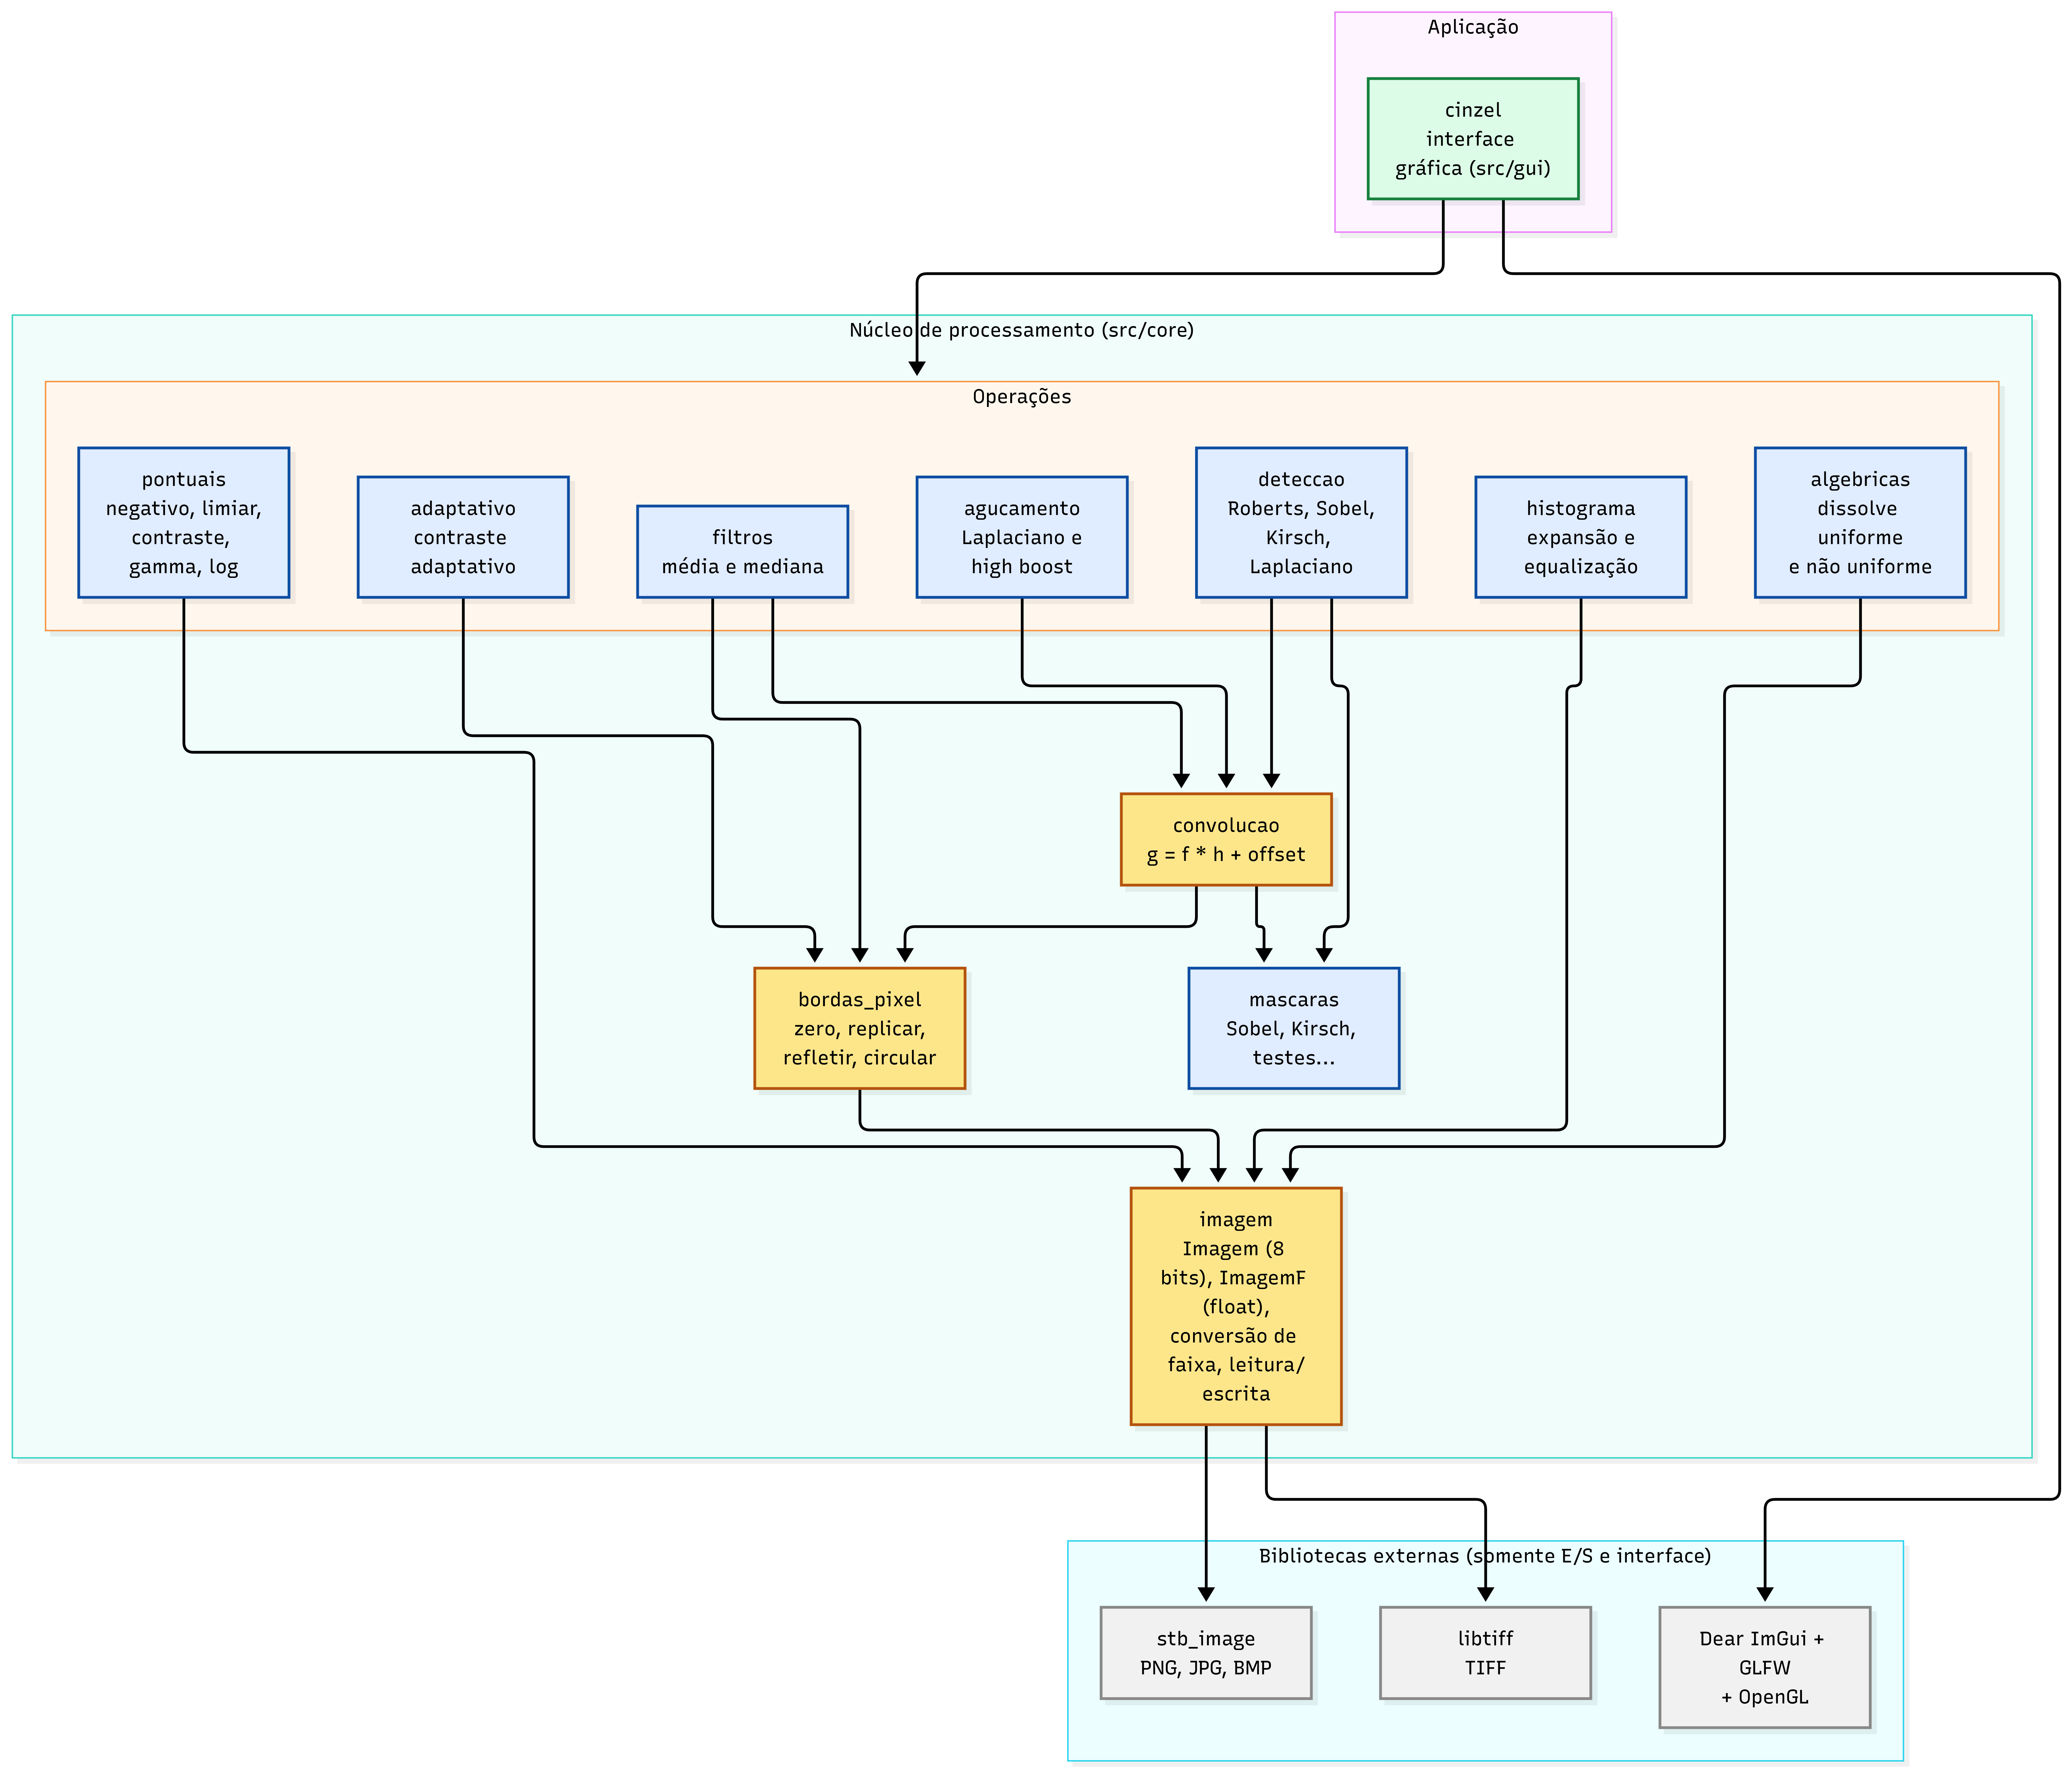
\includegraphics[width=0.8\textwidth]{arquitetura.png}
\caption{Arquitetura da aplicação: a interface depende apenas do núcleo de processamento, e as
operações de vizinhança dependem da convolução e do acesso a pixels com tratamento de bordas.}
\label{fig:arquitetura}
\end{figure}

\subsection{Implementação das operações}

Duas decisões atravessam todas as operações:
\begin{itemize}
  \item \textbf{Tratamento das bordas.} Toda leitura de vizinhança passa pela função
        \texttt{pixelComBorda}, que implementa as estratégias zero, replicação, reflexão e
        circular. A estratégia é um parâmetro de todas as operações de vizinhança e pode ser
        escolhida na interface; nos resultados deste relatório foi usada a replicação, exceto
        no teste específico de bordas.
  \item \textbf{Valores fora de $[0, 255]$.} Operações que podem gerar esses valores são
        calculadas em \texttt{ImagemF} e só convertidas para 8 bits no final, por uma
        estratégia explícita: \textbf{saturação}, $v' = \mathrm{clamp}(v, 0, 255)$;
        \textbf{normalização}, $v' = 255 (v - v_{\min})/(v_{\max} - v_{\min})$; ou
        \textbf{valor absoluto}, $v' = \min(|v|, 255)$. Nunca é feita a conversão direta para
        \texttt{uint8\_t}, que reduziria o valor módulo 256 (por exemplo, $-160 \mapsto 96$ e
        $300 \mapsto 44$). A normalização trata a imagem constante ($v_{\max} = v_{\min}$) sem
        divisão por zero.
\end{itemize}

\subsubsection{Operações algébricas e transformações de intensidade}

O dissolve uniforme percorre os pixels calculando $(1-t) f_1 + t f_2$ e arredondando o
resultado. O não uniforme recebe uma \texttt{ImagemF} de pesos $t(x, y) \in [0, 1]$; foram
implementados geradores de pesos em rampa horizontal, $t = x/(M-1)$, e radial,
$t = d(x,y)/d_{\max}$, em que $d$ é a distância ao centro. As duas imagens precisam ter o mesmo
tamanho; caso contrário, a função lança uma exceção, que a interface exibe como mensagem.

Como as transformações de intensidade dependem apenas do valor do pixel, todas foram
implementadas por meio de uma \textbf{tabela de consulta} (LUT) de 256 posições: calcula-se
$\texttt{lut}[r] = T(r)$ para $r = 0, \dots, 255$ uma única vez e depois aplica-se
$s = \texttt{lut}[r]$ a cada pixel. Os parâmetros são: o limiar $T$ (limiarização); os pontos
$(r_1, s_1)$ e $(r_2, s_2)$ (alargamento, com as divisões protegidas nos casos $r_1 = 0$,
$r_1 = r_2$ e $r_2 = 255$); $c$ e $\gamma$ (potência, com normalização de $r$ para $[0,1]$); e
$c$ (logaritmo, com valor automático $255/\ln 256$ quando $c = 0$). Os resultados são
arredondados e saturados em $[0, 255]$.

\subsubsection{Expansão e equalização de histograma}

O histograma é um vetor de 256 contadores preenchido em uma única passagem pela imagem. A
expansão encontra $r_{\min}$ e $r_{\max}$ e monta a LUT linear da expansão (Seção~2.3); se a
imagem for constante, ela é devolvida sem alteração. A equalização acumula $p(k) = h(k)/N$ em
ordem crescente de $k$ e monta a LUT $s_k = \mathrm{round}(255 \cdot \mathrm{CDF}(k))$. Para o
relatório, foi implementada também uma função que desenha o histograma como imagem (barras
pretas em fundo branco, com altura normalizada pelo maior valor).

\subsubsection{Filtros da média e mediana}

O filtro da média é implementado como uma convolução com a máscara $n \times n$ de
coeficientes $1/n^2$, reutilizando a convolução genérica. O filtro da mediana percorre, para
cada pixel, a vizinhança $n \times n$ centrada nele, lendo cada vizinho por
\texttt{pixelComBorda} e guardando-o em um vetor. A mediana é obtida com
\texttt{std::nth\_element}, que posiciona o elemento central como se o vetor estivesse
ordenado, sem ordenar o restante. Nos dois filtros, $n$ é parametrizável e a interface
restringe $n$ a valores ímpares, para que a vizinhança tenha um centro exato.

\subsubsection{Convolução genérica}

A convolução recebe a imagem $f$, a máscara $h$ de dimensão $n \times m$ (digitada na
interface em uma grade de até $9 \times 9$ ou carregada de uma das máscaras prontas), o
offset, a estratégia de borda, a estratégia de faixa e uma opção que define se a máscara é
rotacionada. O centro da máscara fica em $\big(\lfloor (n-1)/2 \rfloor,
\lfloor (m-1)/2 \rfloor\big)$: para dimensões ímpares é o centro exato; para dimensões pares
(como o Roberts $2 \times 2$) fica no canto superior esquerdo do bloco central. O trecho
essencial é:

\begin{verbatim}
for (int y = 0; y < f.altura; ++y)
  for (int x = 0; x < f.largura; ++x) {
    float soma = 0.0f;
    for (int i = 0; i < h.linhas; ++i)
      for (int j = 0; j < h.colunas; ++j) {
        int s = i - cy, t = j - cx;  // deslocamento ao centro
        // convolucao: f(x - t, y - s);  correlacao: f(x + t, y + s)
        float valor = rotacionar ? pixelComBorda(f, x - t, y - s, borda)
                                 : pixelComBorda(f, x + t, y + s, borda);
        soma += h.at(i, j) * valor;
      }
    g.at(x, y) = soma;
  }
\end{verbatim}

O resultado é acumulado em \texttt{float}; em seguida o offset é somado e a imagem é
convertida para 8 bits pela estratégia de faixa escolhida, ou seja,
$g = \mathrm{Faixa}(f * h + \text{offset})$. Na convolução genérica, a opção padrão é a
convolução verdadeira (máscara rotacionada em $180^\circ$), conforme a definição
$g = f * h$; a correlação pode ser selecionada para comparação.

\subsubsection{Roberts, Sobel, Kirsch e Laplaciano}

Os detectores reutilizam a função de convolução, aplicando as máscaras por
\textbf{correlação}, isto é, exatamente como estão escritas. Assim, $G_x > 0$ indica que a
intensidade cresce para a direita, $G_y > 0$ que cresce para baixo, e a máscara $K_0$ do
Kirsch responde a regiões claras acima do pixel.

\begin{itemize}
  \item \textbf{Roberts e Sobel:} calculam $G_x$ e $G_y$ em \texttt{ImagemF} e combinam as
        componentes pela magnitude euclidiana ou pela soma dos valores absolutos (opção da
        interface). $G_x$ e $G_y$ são exibidos normalizados, de modo que o cinza médio
        representa zero, tons escuros os valores negativos e tons claros os positivos; a
        magnitude é saturada (ou tratada pela estratégia escolhida).
  \item \textbf{Kirsch:} as oito máscaras são geradas por código, deslocando circularmente os
        valores do anel externo da máscara $K_0$ ($[5, 5, 5, -3, -3, -3, -3, -3]$, no sentido
        horário). Cada máscara é aplicada, sua resposta é guardada como imagem intermediária
        (nomeada pela direção: N, NE, L, SE, S, SO, O, NO) e a resposta final é o máximo
        pixel a pixel das oito respostas.
  \item \textbf{Laplaciano:} aplica a máscara de 4 ou 8 vizinhos e exibe a resposta
        normalizada (que mostra o sinal) e a resposta pela estratégia escolhida (por padrão,
        valor absoluto).
\end{itemize}

\subsubsection{Aguçamento e high boost}

O aguçamento calcula o Laplaciano em \texttt{ImagemF}, determina $c$ pelo sinal do
coeficiente central da máscara ($c = -1$ para centro negativo) e soma $c\,\nabla^2 f$ à imagem
original, também em \texttt{ImagemF}. Só então o resultado é saturado. A resposta do
Laplaciano é exibida separadamente, em versão normalizada e em valor absoluto, junto da imagem
aguçada.

O \textit{high boost} suaviza a imagem com o filtro da média $n \times n$, calcula a máscara de
nitidez $f - \bar f$ (com valores positivos e negativos) e soma $k (f - \bar f)$ à original.
São exibidas a imagem suavizada, a máscara de nitidez normalizada e o resultado.

\subsubsection{Controle de contraste adaptativo}

Para cada pixel, a vizinhança $n \times n$ é percorrida uma vez, acumulando a soma
$\sum \tilde f$ e a soma dos quadrados $\sum \tilde f^2$. A média é $m = \sum \tilde f / N$ e
a variância é $\sigma^2 = \sum \tilde f^2 / N - m^2$, limitada inferiormente a zero para
evitar raiz de valores negativos causados por arredondamento. O pixel de saída é
$m + (c / \sigma)(f - m)$, ou o próprio $f$ quando $\sigma \approx 0$. O resultado é saturado
em $[0, 255]$. A constante $c$ e a dimensão $n$ são parâmetros, e a média e o desvio padrão
locais são exibidos como imagens intermediárias.

\subsection{Validação}

O executável \texttt{cinzel\_testes} executa 82 verificações automáticas, cada uma comparando
a saída do sistema com um valor calculado manualmente em uma matriz pequena. Alguns exemplos:
\begin{itemize}
  \item Laplaciano de 4 vizinhos no centro de uma matriz $3 \times 3$ com valor 50 cercado
        por 10: $4 \cdot 10 - 4 \cdot 50 = -160$; o aguçamento resulta em $50 + 160 = 210$.
  \item Sobel em uma borda vertical (colunas 10, 10 e 100): $G_x = 90 + 2 \cdot 90 + 90 = 360$,
        $G_y = 0$ e magnitude saturada em 255; no Kirsch, a máscara $K_2$ (Leste) vence com
        resposta 1350.
  \item Média e mediana de uma vizinhança com um pixel 255 cercado por 10: média
        $335/9 \approx 37$ e mediana 10.
  \item Uma máscara que desloca a imagem diferencia convolução e correlação: no mesmo pixel,
        a convolução lê o vizinho da esquerda e a correlação o da direita.
  \item Equalização de 16 pixels (seis com valor 2, seis com 3, quatro com 5): os níveis são
        mapeados em $\mathrm{round}(255 \cdot 6/16) = 96$, $191$ e $255$.
\end{itemize}
Todas as verificações passam. A leitura de TIFF foi conferida comparando os pixels obtidos
com os da biblioteca Python Pillow nas 38 imagens TIFF de teste, com diferença nula em todas.

% ============================================================
% 4 RESULTADOS
% ============================================================
\section{Resultados}

Todas as imagens desta seção foram geradas pelo executável \texttt{cinzel\_relatorio}, que
aplica as mesmas funções usadas pela interface. Salvo indicação contrária, as operações de
vizinhança usam borda por replicação.

\subsection{Interface e fluxo de utilização}

A interface (Figura~\ref{fig:interface}) é dividida em duas áreas. À esquerda fica o painel de
controle, onde o usuário escolhe a imagem de entrada (lista dos arquivos da pasta de imagens,
incluindo TIFF), seleciona uma das 19 operações e ajusta os parâmetros por controles
deslizantes. Com a opção ``Aplicar automaticamente'', o resultado é recalculado a cada
alteração de parâmetro, o que permite observar o efeito de $\gamma$, $T$, $c$ ou $n$ em tempo
real. Para operações de vizinhança há um seletor da estratégia de borda; para a convolução
genérica, uma grade editável de até $9 \times 9$ coeficientes, campos de offset e estratégia de
faixa, a opção de rotacionar a máscara e botões com as máscaras dos testes obrigatórios. O
dissolve exibe um segundo seletor de arquivo para $f_2$.

À direita são exibidas a imagem original e o resultado, cada uma com o seu histograma, e
abaixo as respostas intermediárias da operação ($G_x$, $G_y$ e magnitude; as oito respostas do
Kirsch e o máximo; a resposta do Laplaciano e a imagem aguçada; etc.). Ao posicionar o mouse
sobre qualquer imagem, o sistema mostra as coordenadas, o valor do pixel e a vizinhança
$3 \times 3$, o que permite conferir manualmente um cálculo. O botão ``Usar resultado como
entrada'' encadeia operações, e ``Salvar resultado e respostas'' grava todas as imagens
exibidas.

\begin{figure}[H]
\centering
% Salve a captura em imagens/interface.png, apague a caixa abaixo e descomente:
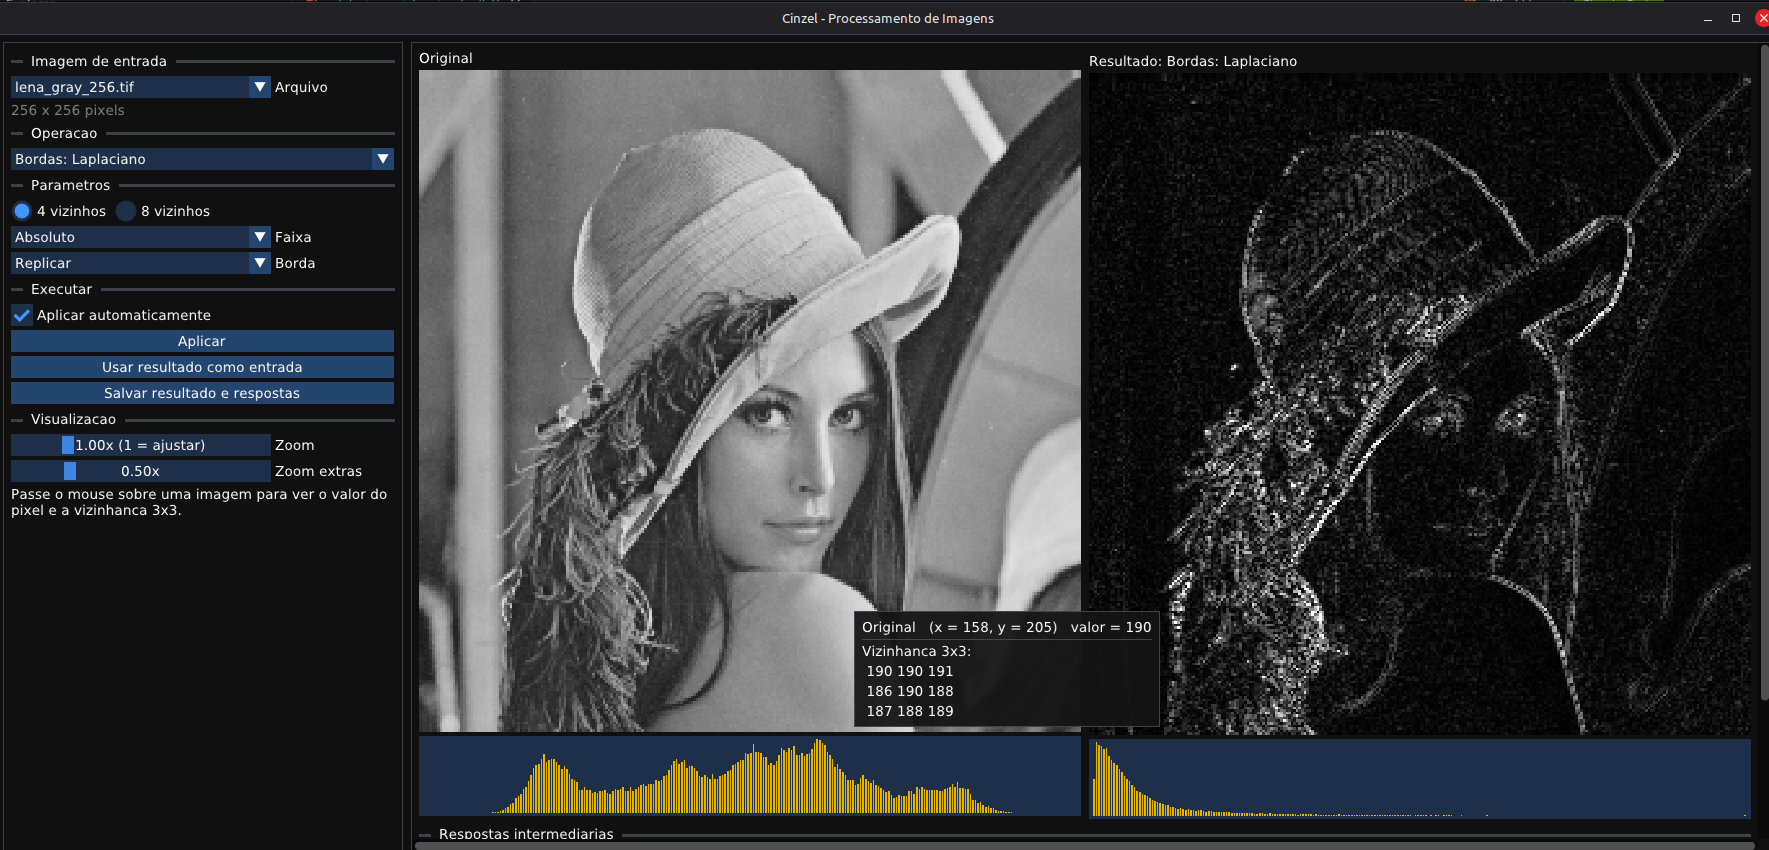
\includegraphics[width=\textwidth]{aplicacao.png}
\caption{Interface principal do sistema desenvolvido.}
\label{fig:interface}
\end{figure}

\subsection{Transformações de intensidade e histogramas}

\textbf{Dissolve cruzado.} A Figura~\ref{fig:dissolve} mostra o dissolve entre a Lena ($f_1$) e
o Mandril ($f_2$). No uniforme, a imagem dominante passa gradualmente de $f_1$ para $f_2$
conforme $t$ cresce, e em $t = 0{,}5$ as duas aparecem com o mesmo peso. No não uniforme, a
transição é espacial: com a rampa, $f_1$ domina à esquerda e $f_2$ à direita; com o padrão
radial, $f_1$ permanece no centro e $f_2$ aparece nos cantos.

\begin{figure}[H]
\centering
\celula{0.18}{01_algebricas/original_f1.png}{$f_1$}\hfill
\celula{0.18}{01_algebricas/dissolve_uniforme_t025.png}{$t = 0{,}25$}\hfill
\celula{0.18}{01_algebricas/dissolve_uniforme_t05.png}{$t = 0{,}5$}\hfill
\celula{0.18}{01_algebricas/dissolve_uniforme_t075.png}{$t = 0{,}75$}\hfill
\celula{0.18}{01_algebricas/original_f2.png}{$f_2$}\\[2mm]
\celula{0.18}{01_algebricas/pesos_rampa.png}{pesos: rampa}\hspace{2mm}
\celula{0.18}{01_algebricas/dissolve_nao_uniforme_rampa.png}{não uniforme: rampa}\hspace{6mm}
\celula{0.18}{01_algebricas/pesos_radial.png}{pesos: radial}\hspace{2mm}
\celula{0.18}{01_algebricas/dissolve_nao_uniforme_radial.png}{não uniforme: radial}
\caption{Dissolve cruzado uniforme (primeira linha) e não uniforme (segunda linha). Nos mapas
de pesos, preto corresponde a $t = 0$ e branco a $t = 1$.}
\label{fig:dissolve}
\end{figure}

\textbf{Negativo, alargamento de contraste e limiarização.} No negativo da mamografia
(Figura~\ref{fig:pontuais}), o tecido denso, antes claro, passa a escuro sobre fundo claro,
evidenciando estruturas sutis. A imagem \textit{polymersomes} ocupa só a faixa $[90, 241]$;
o alargamento com $(r_1, s_1) = (140, 30)$ e $(r_2, s_2) = (200, 230)$ aplica inclinação
$200/60 \approx 3{,}3$ à faixa central, onde está a maioria dos pixels, e torna nítidas as
bordas das vesículas. Na limiarização, $T$ define o que é considerado objeto: $T = 60$ mantém
quase toda a face em branco, $T = 128$ separa as regiões claras e escuras, e $T = 180$ preserva
apenas as regiões mais claras.

\begin{figure}[H]
\centering
\celula{0.15}{02_intensidade/negativo_original.png}{mamografia}\hfill
\celula{0.15}{02_intensidade/negativo_resultado.png}{negativo}\hfill
\celula{0.13}{02_intensidade/negativo_curva.png}{$s = 255 - r$}\hfill
\celula{0.17}{02_intensidade/contraste_original.png}{polymersomes}\hfill
\celula{0.17}{02_intensidade/contraste_resultado.png}{alargamento}\hfill
\celula{0.13}{02_intensidade/contraste_curva.png}{curva}\\[2mm]
\celula{0.22}{02_intensidade/limiar_original.png}{original}\hfill
\celula{0.22}{02_intensidade/limiar_T60.png}{$T = 60$}\hfill
\celula{0.22}{02_intensidade/limiar_T128.png}{$T = 128$}\hfill
\celula{0.22}{02_intensidade/limiar_T180.png}{$T = 180$}
\caption{Negativo, alargamento de contraste (com as curvas $s = T(r)$; a diagonal cinza é a
identidade) e limiarização com três limiares.}
\label{fig:pontuais}
\end{figure}

\textbf{Potência (gamma).} Antes de executar o teste na ressonância da coluna, foi feita uma
previsão qualitativa do efeito de passar $\gamma$ de 1 para $0{,}5$. A imagem é
predominantemente escura: 76\% dos pixels estão abaixo de 32 e a mediana é 1. Com
$\gamma = 0{,}5$, a curva $s = 255\sqrt{r/255}$ fica acima da identidade e tem inclinação muito
maior que 1 perto de $r = 0$, menor que 1 perto de $r = 255$. Esperava-se, portanto, que (i) a
imagem clareasse de forma geral; (ii) os tons escuros fossem expandidos, revelando estruturas
antes escondidas nas sombras; (iii) os tons claros fossem comprimidos, reduzindo o contraste
entre eles; e (iv) o ruído quase preto do fundo fosse amplificado. Numericamente, a curva leva
$1 \mapsto 16$, $64 \mapsto 128$ e $200 \mapsto 226$: um pixel escuro ganha 64 níveis e um claro,
apenas 26.

O resultado (Figura~\ref{fig:gamma}) confirma a previsão: com $\gamma = 0{,}5$ a média passa de
32,6 para 59,2 e a mediana de 1 para 16, exatamente o valor previsto para $r = 1$. As vértebras
e os tecidos ao redor da coluna tornam-se visíveis, e o fundo deixa de ser preto uniforme. A
sequência $\gamma = 0{,}6$, $0{,}5$, $0{,}4$ e $0{,}3$ eleva a média para 50,1, 59,2, 72,5 e
92,1. Com $\gamma = 0{,}3$, o fundo fica acinzentado (apenas 1,5\% dos pixels permanecem abaixo
de 32), o que mostra a amplificação do ruído escuro. Na foto aérea ``lavada'' (média 197,1),
$\gamma > 1$ tem o efeito oposto: escurece a imagem (média 131,5 para $\gamma = 3$ e 94,7 para
$\gamma = 5$) e recupera o contraste das regiões claras.

\begin{figure}[H]
\centering
\celula{0.15}{02_intensidade/gamma_escura_original.png}{original ($\gamma = 1$)}\hfill
\celula{0.15}{02_intensidade/gamma_escura_g06.png}{$\gamma = 0{,}6$}\hfill
\celula{0.15}{02_intensidade/gamma_escura_g05.png}{$\gamma = 0{,}5$}\hfill
\celula{0.15}{02_intensidade/gamma_escura_g04.png}{$\gamma = 0{,}4$}\hfill
\celula{0.15}{02_intensidade/gamma_escura_g03.png}{$\gamma = 0{,}3$}\hfill
\celula{0.13}{02_intensidade/gamma_curva_g05.png}{curva $\gamma = 0{,}5$}\\[2mm]
\celula{0.18}{02_intensidade/gamma_clara_original.png}{original ($\gamma = 1$)}\hfill
\celula{0.18}{02_intensidade/gamma_clara_g3.png}{$\gamma = 3$}\hfill
\celula{0.18}{02_intensidade/gamma_clara_g4.png}{$\gamma = 4$}\hfill
\celula{0.18}{02_intensidade/gamma_clara_g5.png}{$\gamma = 5$}\hfill
\celula{0.13}{02_intensidade/gamma_curva_g3.png}{curva $\gamma = 3$}
\caption{Transformação de potência com $c = 1$ em uma imagem predominantemente escura
($\gamma < 1$, primeira linha) e em uma imagem predominantemente clara ($\gamma > 1$, segunda
linha). A diagonal cinza das curvas é a identidade ($\gamma = 1$).}
\label{fig:gamma}
\end{figure}

\textbf{Logaritmo.} Aplicado à imagem do Hubble (Figura~\ref{fig:log}), o logaritmo com
$c = 255/\ln 256$ eleva a média de 34,5 para 160,1 e torna visíveis galáxias tênues. Ao mesmo
tempo, reduz o desvio padrão de 25,1 para 15,2: os tons claros são comprimidos, e as estrelas
mais brilhantes perdem contraste entre si.

\begin{figure}[H]
\centering
\celula{0.28}{02_intensidade/log_original.png}{original}\hspace{4mm}
\celula{0.28}{02_intensidade/log_resultado.png}{logaritmo}\hspace{4mm}
\celula{0.2}{02_intensidade/log_curva.png}{curva $s = c\ln(1+r)$}
\caption{Transformação logarítmica com $c = 255/\ln 256 \approx 45{,}99$.}
\label{fig:log}
\end{figure}

\textbf{Expansão e equalização de histograma.} A Tabela~\ref{tab:histograma} resume as
estatísticas e a Figura~\ref{fig:histograma} mostra as imagens com seus histogramas. Na
\textit{polymersomes}, a expansão leva $[90, 241]$ para $[0, 255]$, multiplicando o desvio
padrão pelo fator $255/151 \approx 1{,}7$ sem alterar o número de níveis (152) nem a forma do
histograma. A equalização espalha os níveis pela escala inteira e eleva o desvio padrão para
73,0, mas funde níveis vizinhos (restam 69) e realça também a textura do fundo. Na
\textit{sol2}, que já ocupa a faixa $[0, 249]$, a expansão quase não muda nada, enquanto a
equalização eleva a média de 34,4 para 130,7. Na imagem \textit{regiao}, que tem apenas dois
níveis (127 em 70,6\% dos pixels e 204 nos demais), a expansão produz 0 e 255, mas a
equalização produz 180 e 255: o nível mais frequente recebe
$\mathrm{round}(255 \cdot 0{,}706) = 180$, e o histograma continua com duas barras.

\begin{table}[H]
\centering
\small
\begin{tabular}{llrrrrr}
\toprule
\textbf{Imagem} & \textbf{Operação} & \textbf{mín.} & \textbf{máx.} & \textbf{média} & \textbf{desvio} & \textbf{níveis} \\
\midrule
polymersomes & original    & 90  & 241 & 169,6 & 13,8  & 152 \\
             & expansão    & 0   & 255 & 134,5 & 23,3  & 152 \\
             & equalização & 0   & 255 & 133,4 & 73,0  & 69  \\
\midrule
regiao       & original    & 127 & 204 & 149,7 & 35,1  & 2 \\
             & expansão    & 0   & 255 & 75,1  & 116,2 & 2 \\
             & equalização & 180 & 255 & 202,1 & 34,2  & 2 \\
\midrule
sol2         & original    & 0   & 249 & 34,4  & 39,6  & 202 \\
             & expansão    & 0   & 255 & 35,1  & 40,6  & 202 \\
             & equalização & 26  & 255 & 130,7 & 70,3  & 118 \\
\midrule
washed       & original    & 0   & 255 & 197,1 & 40,9  & 236 \\
             & equalização & 0   & 255 & 128,7 & 73,9  & 133 \\
\bottomrule
\end{tabular}
\caption{Estatísticas das imagens antes e depois da expansão e da equalização.}
\label{tab:histograma}
\end{table}

\begin{figure}[H]
\centering
\celula{0.15}{03_histograma/polymersomes_original.png}{polymersomes}\hfill
\celula{0.15}{03_histograma/polymersomes_expansao.png}{expansão}\hfill
\celula{0.15}{03_histograma/polymersomes_equalizacao.png}{equalização}\hfill
\celula{0.15}{03_histograma/sol2_original.png}{sol2}\hfill
\celula{0.15}{03_histograma/sol2_expansao.png}{expansão}\hfill
\celula{0.15}{03_histograma/sol2_equalizacao.png}{equalização}\\[1mm]
\celula{0.15}{03_histograma/polymersomes_original_hist.png}{}\hfill
\celula{0.15}{03_histograma/polymersomes_expansao_hist.png}{}\hfill
\celula{0.15}{03_histograma/polymersomes_equalizacao_hist.png}{}\hfill
\celula{0.15}{03_histograma/sol2_original_hist.png}{}\hfill
\celula{0.15}{03_histograma/sol2_expansao_hist.png}{}\hfill
\celula{0.15}{03_histograma/sol2_equalizacao_hist.png}{}\\[2mm]
\celula{0.15}{03_histograma/regiao_original.png}{regiao}\hfill
\celula{0.15}{03_histograma/regiao_expansao.png}{expansão}\hfill
\celula{0.15}{03_histograma/regiao_equalizacao.png}{equalização}\hfill
\celula{0.15}{03_histograma/washed_original.png}{washed}\hfill
\celula{0.15}{03_histograma/washed_equalizacao.png}{equalização}\hfill
\begin{minipage}[t]{0.15\textwidth}\hfill\end{minipage}\\[1mm]
\celula{0.15}{03_histograma/regiao_original_hist.png}{}\hfill
\celula{0.15}{03_histograma/regiao_expansao_hist.png}{}\hfill
\celula{0.15}{03_histograma/regiao_equalizacao_hist.png}{}\hfill
\celula{0.15}{03_histograma/washed_original_hist.png}{}\hfill
\celula{0.15}{03_histograma/washed_equalizacao_hist.png}{}\hfill
\begin{minipage}[t]{0.15\textwidth}\hfill\end{minipage}
\caption{Expansão e equalização de histograma. Abaixo de cada imagem está o seu histograma
(eixo horizontal: níveis 0 a 255).}
\label{fig:histograma}
\end{figure}

\subsection{Filtragem espacial}

Para comparar os filtros, foi adicionado 5\% de ruído sal-e-pimenta (2,5\% de pixels com 0 e
2,5\% com 255, semente fixa) à Lena $256 \times 256$. A Tabela~\ref{tab:psnr} mede a
fidelidade de cada resultado à imagem original pela PSNR,
$\mathrm{PSNR} = 10 \log_{10}(255^2/\mathrm{MSE})$, em que valores maiores indicam maior
semelhança. A imagem ruidosa tem PSNR de 18,4~dB. A mediana $3 \times 3$ remove praticamente
todo o ruído (29,6~dB) e preserva as bordas, enquanto a média $3 \times 3$ transforma cada
impulso em uma mancha cinza (25,0~dB). Aumentar $n$ piora os dois filtros, porque a suavização
passa a apagar detalhes da própria imagem (Figura~\ref{fig:filtros}).

\begin{table}[H]
\centering
\small
\begin{tabular}{lccc}
\toprule
\textbf{Filtro} & $n = 3$ & $n = 5$ & $n = 7$ \\
\midrule
Média   & 25,02 dB & 24,61 dB & 23,57 dB \\
Mediana & 29,58 dB & 27,12 dB & 25,62 dB \\
\bottomrule
\end{tabular}
\caption{PSNR em relação à imagem original sem ruído (imagem ruidosa: 18,42 dB).}
\label{tab:psnr}
\end{table}

\begin{figure}[H]
\centering
\celula{0.18}{05_filtragem/original.png}{original}\hfill
\celula{0.18}{05_filtragem/ruido_sal_pimenta.png}{com ruído (5\%)}\hfill
\celula{0.18}{05_filtragem/media_n3.png}{média $3 \times 3$}\hfill
\celula{0.18}{05_filtragem/media_n5.png}{média $5 \times 5$}\hfill
\celula{0.18}{05_filtragem/media_n7.png}{média $7 \times 7$}\\[2mm]
\begin{minipage}[t]{0.18\textwidth}\hfill\end{minipage}\hfill
\begin{minipage}[t]{0.18\textwidth}\hfill\end{minipage}\hfill
\celula{0.18}{05_filtragem/mediana_n3.png}{mediana $3 \times 3$}\hfill
\celula{0.18}{05_filtragem/mediana_n5.png}{mediana $5 \times 5$}\hfill
\celula{0.18}{05_filtragem/mediana_n7.png}{mediana $7 \times 7$}
\caption{Filtros da média e da mediana aplicados à imagem com ruído sal-e-pimenta.}
\label{fig:filtros}
\end{figure}

O efeito do tratamento das bordas fica evidente com uma janela grande
(Figura~\ref{fig:bordas-estrategias}). Com a média $25 \times 25$ e borda zero, os pixels
fictícios valem 0 e escurecem uma faixa de 12 pixels em toda a moldura. Com replicação e
reflexão a moldura mantém a intensidade das regiões vizinhas. Com a estratégia circular, cada
borda recebe valores do lado oposto da imagem, o que mistura o céu claro do topo com o gramado
da base.

\begin{figure}[H]
\centering
\celula{0.18}{05_filtragem/bordas_original.png}{original}\hfill
\celula{0.18}{05_filtragem/bordas_media25_zero.png}{zero}\hfill
\celula{0.18}{05_filtragem/bordas_media25_replicar.png}{replicação}\hfill
\celula{0.18}{05_filtragem/bordas_media25_refletir.png}{reflexão}\hfill
\celula{0.18}{05_filtragem/bordas_media25_circular.png}{circular}
\caption{Média $25 \times 25$ com as quatro estratégias de tratamento das bordas.}
\label{fig:bordas-estrategias}
\end{figure}

\subsection{Testes de convolução}

Todos os testes desta seção usam a convolução genérica com a máscara rotacionada em
$180^\circ$ (convolução verdadeira), borda por replicação e a imagem \textit{cameraman}.

\subsubsection{Filtro de aguçamento}

A máscara do teste é
\begin{equation}
  h = \begin{bmatrix} -c & -c & -c \\ -c & 8c + d & -c \\ -c & -c & -c \end{bmatrix},
  \qquad \sum h = -8c + (8c + d) = d.
\end{equation}
Ela pode ser decomposta como $h = d\,\delta + c\,L$, em que $\delta$ é a máscara identidade e
$L$ é o negativo do Laplaciano de 8 vizinhos (centro 8, vizinhos $-1$, soma 0). Assim,
$g = d \cdot f + c \cdot (\text{realce de bordas})$: o parâmetro $d$ controla o peso da imagem
original e, portanto, o brilho médio, e $c$ controla a intensidade do realce das bordas. Os
resultados foram saturados em $[0, 255]$ e estão na Figura~\ref{fig:t21} e na
Tabela~\ref{tab:t21}.

Com $c = d = 1$, a soma é 1: a média permanece praticamente igual à da original (121,1 contra
118,7), e o desvio padrão sobe de 62,3 para 82,6, refletindo bordas mais marcadas. Com
$c = 1$ e $d$ crescente, a soma passa a ser $d$ e a imagem é multiplicada por $d$ nas regiões
uniformes: com $d = 2$, 60,6\% dos pixels já saturam em 255 e, com $d = 4$, 73,4\% e restam praticamente só as regiões
escuras. Com $d = 1$ e $c$ crescente, a média se mantém (soma 1), mas o realce fica cada vez
mais forte: com $c = 3$, 15,6\% dos pixels saturam em 255 e 21,2\% em 0, e a textura do
gramado e o ruído aparecem amplificados.

\begin{table}[H]
\centering
\small
\begin{tabular}{cccccccc}
\toprule
$c$ & $d$ & centro & $\sum h$ & média & desvio & pixels em 255 & pixels em 0 \\
\midrule
\multicolumn{4}{l}{original} & 118,7 & 62,3 & -- & -- \\
1 & 1 & 9  & 1 & 121,1 & 82,6  & 7,3\%  & 11,8\% \\
1 & 2 & 10 & 2 & 183,7 & 102,1 & 60,6\% & 7,1\% \\
1 & 4 & 12 & 4 & 203,7 & 90,5  & 73,4\% & 4,3\% \\
2 & 1 & 17 & 1 & 122,2 & 90,4  & 11,8\% & 17,8\% \\
3 & 1 & 25 & 1 & 122,7 & 95,4  & 15,6\% & 21,2\% \\
\bottomrule
\end{tabular}
\caption{Estatísticas do teste de aguçamento (resultados saturados em $[0,255]$).}
\label{tab:t21}
\end{table}

\begin{figure}[H]
\centering
\celula{0.155}{08_testes_convolucao/original.png}{original}\hfill
\celula{0.155}{08_testes_convolucao/t21_c1_d1.png}{$c = 1$, $d = 1$}\hfill
\celula{0.155}{08_testes_convolucao/t21_c1_d2.png}{$c = 1$, $d = 2$}\hfill
\celula{0.155}{08_testes_convolucao/t21_c1_d4.png}{$c = 1$, $d = 4$}\hfill
\celula{0.155}{08_testes_convolucao/t21_c2_d1.png}{$c = 2$, $d = 1$}\hfill
\celula{0.155}{08_testes_convolucao/t21_c3_d1.png}{$c = 3$, $d = 1$}
\caption{Teste 2.1: filtro de aguçamento com diferentes valores de $c$ e $d$.}
\label{fig:t21}
\end{figure}

\subsubsection{Filtros de relevo}

As máscaras do teste são
\begin{equation}
  h_1 = \begin{bmatrix} 0 & 0 & 0 \\ 0 & 1 & 0 \\ 0 & 0 & -1 \end{bmatrix}, \qquad
  h_2 = \begin{bmatrix} 0 & 0 & 2 \\ 0 & -1 & 0 \\ -1 & 0 & 0 \end{bmatrix},
\end{equation}
ambas com soma zero. Por isso, regiões uniformes produzem resposta nula e foi usado offset 128,
de modo que o cinza médio represente ``sem variação'', tons claros as variações positivas e
tons escuros as negativas (Figura~\ref{fig:t22}).

Com a rotação da convolução, $h_1$ calcula $g = f(x, y) - f(x-1, y-1)$: a diferença entre o
pixel e o seu vizinho diagonal superior esquerdo. Bordas em que a intensidade cresce no sentido
da diagonal principal ficam claras e as de sentido oposto ficam escuras, o que produz a ilusão
de uma superfície em relevo iluminada obliquamente. A máscara $h_2$ atua na outra diagonal
(do canto inferior esquerdo ao superior direito), com $g = 2f(x-1, y+1) - f(x, y) - f(x+1, y-1)$.
Por isso as bordas realçadas e a direção aparente da iluminação mudam, e o peso 2 produz um
relevo mais intenso: o desvio padrão é 40,0, contra 24,6 de $h_1$. Bordas paralelas à diagonal
de cada máscara praticamente não aparecem, pois não há variação na direção analisada.

Sem offset, a saturação elimina todas as respostas negativas e restam apenas as bordas de um
dos lados. A versão por correlação (máscara não rotacionada) inverte o sentido das diferenças:
regiões que eram claras ficam escuras e vice-versa, e o relevo parece ``afundado'' em vez de
``elevado''. Isso mostra que a orientação dos coeficientes, e não apenas os seus valores,
define a aparência do relevo.

\begin{figure}[H]
\centering
\celula{0.155}{08_testes_convolucao/t22_h1_offset128.png}{$h_1$, offset 128}\hfill
\celula{0.155}{08_testes_convolucao/t22_h1_offset0.png}{$h_1$, offset 0}\hfill
\celula{0.155}{08_testes_convolucao/t22_h1_offset128_correlacao.png}{$h_1$, correlação}\hfill
\celula{0.155}{08_testes_convolucao/t22_h2_offset128.png}{$h_2$, offset 128}\hfill
\celula{0.155}{08_testes_convolucao/t22_h2_offset0.png}{$h_2$, offset 0}\hfill
\celula{0.155}{08_testes_convolucao/t22_h2_offset128_correlacao.png}{$h_2$, correlação}
\caption{Teste 2.2: filtros de relevo com e sem offset, por convolução e por correlação.}
\label{fig:t22}
\end{figure}

\subsubsection{Máscaras de detecção de bordas}

As máscaras do teste são
\begin{equation}
  h_3 = \begin{bmatrix} -1 & -1 & 0 \\ 1 & 0 & 1 \\ 0 & 1 & 1 \end{bmatrix}
  \;\left(\textstyle\sum = 2\right), \qquad
  h_4 = \begin{bmatrix} 0 & -1 & 0 \\ -1 & -4 & -1 \\ 0 & -1 & 0 \end{bmatrix}
  \;\left(\textstyle\sum = -8\right).
\end{equation}
Cada uma foi aplicada com as três estratégias de faixa (Figura~\ref{fig:t23}).

Em $h_3$, os coeficientes negativos estão de um lado da diagonal e os positivos do outro, o que
caracteriza um detector \textbf{direcional}: ele responde a variações ao longo dessa diagonal e
responde pouco a bordas paralelas a ela. Como a soma é 2, porém, a máscara não anula regiões
uniformes: ela devolve aproximadamente o dobro da intensidade local somado ao termo de borda.
Com saturação, a imagem fica muito clara (média 194,2), com as bordas aparecendo como linhas
escuras ou claras conforme o sentido da transição. A normalização mostra o resultado completo,
semelhante a um relevo sobre a própria imagem.

Em $h_4$, todos os coeficientes são negativos ou nulos. A máscara é o negativo de uma média
ponderada com peso total 8: para qualquer imagem não negativa, o resultado é
$\leq 0$ em todos os pixels. Com saturação, a imagem resultante é \textbf{inteiramente preta}
(100\% dos pixels em 0). Com valor absoluto, $|{-8}\bar f|$ ultrapassa 255 sempre que a média
local supera 32, e a imagem fica quase toda branca, com exceção das regiões mais escuras. Só a
normalização revela a estrutura, que corresponde à imagem suavizada e invertida. Comparada ao
Laplaciano $[0, 1, 0;\, 1, -4, 1;\, 0, 1, 0]$, a inversão do sinal dos vizinhos muda a soma de
0 para $-8$ e transforma um detector de bordas isotrópico em um filtro passa-baixa invertido.
Isso mostra que a disposição dos sinais importa mais que o formato da máscara.

\begin{figure}[H]
\centering
\celula{0.155}{08_testes_convolucao/t23_h3_saturar.png}{$h_3$, saturar}\hfill
\celula{0.155}{08_testes_convolucao/t23_h3_absoluto.png}{$h_3$, absoluto}\hfill
\celula{0.155}{08_testes_convolucao/t23_h3_normalizar.png}{$h_3$, normalizar}\hfill
\celula{0.155}{08_testes_convolucao/t23_h4_saturar.png}{$h_4$, saturar}\hfill
\celula{0.155}{08_testes_convolucao/t23_h4_absoluto.png}{$h_4$, absoluto}\hfill
\celula{0.155}{08_testes_convolucao/t23_h4_normalizar.png}{$h_4$, normalizar}
\caption{Teste 2.3: máscaras $h_3$ e $h_4$ com as três estratégias de tratamento de valores
fora de $[0,255]$ (offset 0).}
\label{fig:t23}
\end{figure}

\subsection{Roberts, Sobel, Kirsch e Laplaciano}

Os quatro operadores foram aplicados à \textit{cameraman}
(Figuras~\ref{fig:gradiente} a~\ref{fig:laplaciano}). Em $G_x$ e $G_y$, exibidos normalizados,
o cinza médio corresponde a zero: $G_x$ realça as bordas verticais (o tripé e a lateral do
casaco) e $G_y$ as horizontais (a linha do horizonte e os ombros), com sinais opostos nos dois
lados de cada borda. O Roberts produz bordas finas e de baixa amplitude (apenas 0,1\% dos pixels
saturam na magnitude), porque usa só quatro pixels. O Sobel produz bordas mais espessas e
contínuas (7,9\% saturados). A aproximação $|G_x| + |G_y|$ é visualmente semelhante à magnitude
euclidiana, porém ligeiramente mais intensa.

\begin{figure}[H]
\centering
\celula{0.18}{06_deteccao_bordas/original.png}{original}\hfill
\celula{0.18}{06_deteccao_bordas/roberts_Gx.png}{Roberts $G_x$}\hfill
\celula{0.18}{06_deteccao_bordas/roberts_Gy.png}{Roberts $G_y$}\hfill
\celula{0.18}{06_deteccao_bordas/roberts_Magnitude.png}{Roberts $|\nabla f|$}\hfill
\begin{minipage}[t]{0.18\textwidth}\hfill\end{minipage}\\[2mm]
\begin{minipage}[t]{0.18\textwidth}\hfill\end{minipage}\hfill
\celula{0.18}{06_deteccao_bordas/sobel_Gx.png}{Sobel $G_x$}\hfill
\celula{0.18}{06_deteccao_bordas/sobel_Gy.png}{Sobel $G_y$}\hfill
\celula{0.18}{06_deteccao_bordas/sobel_Magnitude.png}{Sobel $\sqrt{G_x^2 + G_y^2}$}\hfill
\celula{0.18}{06_deteccao_bordas/sobel_Magnitude_soma_abs.png}{Sobel $|G_x| + |G_y|$}
\caption{Operadores de Roberts e Sobel: componentes $G_x$ e $G_y$ (normalizadas) e magnitude do
gradiente (saturada).}
\label{fig:gradiente}
\end{figure}

No Kirsch (Figura~\ref{fig:kirsch}), cada máscara realça as bordas de uma orientação: $K_0$ (N)
e $K_4$ (S) acendem nas bordas horizontais, como a linha do horizonte, mas com lados opostos;
$K_2$ (L) e $K_6$ (O) acendem nas verticais, como as pernas do tripé; as diagonais respondem às
bordas inclinadas. A resposta final, o máximo das oito, reúne todas as orientações. Como os
coeficientes (5 e $-3$) produzem respostas grandes, 22,9\% dos pixels saturam e as bordas
ficam espessas; a versão normalizada mostra a variação real de intensidade das bordas.

\begin{figure}[H]
\centering
\celula{0.18}{06_deteccao_bordas/kirsch_K0_N.png}{$K_0$ (N)}\hfill
\celula{0.18}{06_deteccao_bordas/kirsch_K1_NE.png}{$K_1$ (NE)}\hfill
\celula{0.18}{06_deteccao_bordas/kirsch_K2_L.png}{$K_2$ (L)}\hfill
\celula{0.18}{06_deteccao_bordas/kirsch_K3_SE.png}{$K_3$ (SE)}\hfill
\celula{0.18}{06_deteccao_bordas/kirsch_Maximo.png}{máximo (saturado)}\\[2mm]
\celula{0.18}{06_deteccao_bordas/kirsch_K4_S.png}{$K_4$ (S)}\hfill
\celula{0.18}{06_deteccao_bordas/kirsch_K5_SO.png}{$K_5$ (SO)}\hfill
\celula{0.18}{06_deteccao_bordas/kirsch_K6_O.png}{$K_6$ (O)}\hfill
\celula{0.18}{06_deteccao_bordas/kirsch_K7_NO.png}{$K_7$ (NO)}\hfill
\celula{0.18}{06_deteccao_bordas/kirsch_Maximo_normalizado.png}{máximo (normalizado)}
\caption{Operador de Kirsch: respostas das oito máscaras direcionais (valores negativos
saturados em 0) e resposta final.}
\label{fig:kirsch}
\end{figure}

O Laplaciano (Figura~\ref{fig:laplaciano}) responde a todas as orientações ao mesmo tempo. Na
versão normalizada, cada borda aparece como um par de linhas claras e escuras (a dupla resposta
da segunda derivada). Em valor absoluto, as bordas são finas, mas a textura do gramado e o
ruído aparecem com intensidade comparável à dos contornos principais. A máscara de 8 vizinhos
gera respostas mais fortes que a de 4, inclusive para o ruído.

\begin{figure}[H]
\centering
\celula{0.22}{06_deteccao_bordas/laplaciano4_Laplaciano_normalizado.png}{4 vizinhos, normalizado}\hfill
\celula{0.22}{06_deteccao_bordas/laplaciano4_Laplaciano.png}{4 vizinhos, absoluto}\hfill
\celula{0.22}{06_deteccao_bordas/laplaciano8_Laplaciano_normalizado.png}{8 vizinhos, normalizado}\hfill
\celula{0.22}{06_deteccao_bordas/laplaciano8_Laplaciano.png}{8 vizinhos, absoluto}
\caption{Resposta do Laplaciano de 4 e de 8 vizinhos.}
\label{fig:laplaciano}
\end{figure}

\subsection{Aguçamento pelo Laplaciano e high boost}

A Figura~\ref{fig:agucamento} mostra o aguçamento da imagem da Lua por $g = f - \nabla^2 f$. A
resposta do Laplaciano, exibida separadamente, contém apenas as bordas das crateras: o fundo e
as regiões uniformes ficam em zero (cinza médio na versão normalizada e preto na versão
absoluta). Somada à original, essa resposta torna as crateras e a borda do disco mais nítidas
sem perder a informação de fundo. A versão de 8 vizinhos produz um realce mais forte.

No \textit{high boost} da \textit{cameraman}, com média $5 \times 5$, a máscara de nitidez
$f - \bar f$ contém só os detalhes. Com $k = 1$ (\textit{unsharp masking}) o realce é discreto.
Com $k = 2$ e $k = 4$, os contornos ficam progressivamente mais marcados, surgem halos claros e
escuros ao redor das bordas, e a textura do gramado é amplificada.

\begin{figure}[H]
\centering
\celula{0.18}{07_agucamento/lua_original.png}{original}\hfill
\celula{0.18}{07_agucamento/lua_lap4_Laplaciano_normalizado.png}{$\nabla^2 f$ (4 viz.), normalizado}\hfill
\celula{0.18}{07_agucamento/lua_lap4_Laplaciano_absoluto.png}{$|\nabla^2 f|$ (4 viz.)}\hfill
\celula{0.18}{07_agucamento/lua_lap4_Agucada.png}{aguçada (4 viz.)}\hfill
\celula{0.18}{07_agucamento/lua_lap8_Agucada.png}{aguçada (8 viz.)}\\[2mm]
\celula{0.155}{07_agucamento/highboost_original.png}{original}\hfill
\celula{0.155}{07_agucamento/highboost_suavizada.png}{$\bar f$ (média $5 \times 5$)}\hfill
\celula{0.155}{07_agucamento/highboost_mascara_nitidez.png}{$f - \bar f$ (normalizada)}\hfill
\celula{0.155}{07_agucamento/highboost_k1.png}{$k = 1$}\hfill
\celula{0.155}{07_agucamento/highboost_k2.png}{$k = 2$}\hfill
\celula{0.155}{07_agucamento/highboost_k4.png}{$k = 4$}
\caption{Aguçamento pelo Laplaciano (primeira linha), com a resposta do operador exibida
separadamente, e \textit{high boost} (segunda linha).}
\label{fig:agucamento}
\end{figure}

\subsection{Controle de contraste adaptativo}

O contraste adaptativo foi testado na foto \textit{sol2}, escura e com detalhes nas sombras das
árvores (Figura~\ref{fig:adaptativo}). Como a formulação preserva a média local, o brilho geral
praticamente não muda (média entre 35 e 37,5, contra 34,4 na original). O que muda é o contraste
local: texturas da areia e das folhagens, antes uniformes, passam a ser visíveis. Aumentar $c$
de 20 para 40 aumenta o ganho $c/\sigma$ e o desvio padrão global (de 37,1 para 45,1 com
$n = 15$), mas também amplifica o ruído nas regiões quase uniformes. Aumentar $n$ torna as
estatísticas menos locais: com $n = 7$ o realce acompanha detalhes finos, enquanto com $n = 31$
ele passa a refletir regiões maiores. Os mapas de média e desvio padrão locais mostram onde o
ganho é alto (desvio baixo, regiões escuras) e onde é baixo (bordas com o céu).

\begin{figure}[H]
\centering
\celula{0.235}{04_contraste_adaptativo/original.png}{original}\hfill
\celula{0.235}{04_contraste_adaptativo/c20_n7.png}{$c = 20$, $n = 7$}\hfill
\celula{0.235}{04_contraste_adaptativo/c20_n15.png}{$c = 20$, $n = 15$}\hfill
\celula{0.235}{04_contraste_adaptativo/c40_n15.png}{$c = 40$, $n = 15$}\\[2mm]
\celula{0.235}{04_contraste_adaptativo/c40_n31.png}{$c = 40$, $n = 31$}\hfill
\celula{0.235}{04_contraste_adaptativo/c20_n15_media_local.png}{média local ($n = 15$)}\hfill
\celula{0.235}{04_contraste_adaptativo/c20_n15_desvio_local.png}{desvio local ($n = 15$, normalizado)}\hfill
\begin{minipage}[t]{0.235\textwidth}\hfill\end{minipage}
\caption{Controle de contraste adaptativo com diferentes valores de $c$ e $n$, e as estatísticas
locais usadas no cálculo.}
\label{fig:adaptativo}
\end{figure}

% ============================================================
% 5 DISCUSSÃO
% ============================================================
\section{Discussão}

As respostas objetivas às dez questões de domínio conceitual da especificação estão reunidas
no Apêndice~\ref{ap:questoes}; esta seção discute os resultados de forma mais ampla.

\textbf{Operações pontuais e de vizinhança.} As transformações de intensidade, o dissolve, a
expansão e a equalização são pontuais: o valor de saída de um pixel depende apenas do valor
daquele pixel, o que permitiu implementá-las com uma LUT. Na expansão e na equalização, a
função $T$ é calculada a partir de estatísticas globais da imagem ($r_{\min}$, $r_{\max}$ e o
histograma), mas, uma vez calculada, é aplicada a cada pixel de forma independente. Média,
mediana, convolução, detectores de bordas, aguçamento e contraste adaptativo são operações de
vizinhança e, por isso, exigem o tratamento das bordas. O experimento com a média
$25 \times 25$ mostrou que essa escolha não é um detalhe: a borda zero introduz um artefato
visível, e a circular mistura conteúdo de lados opostos da imagem.

\textbf{Média versus mediana.} A diferença de mais de 4~dB na PSNR com $n = 3$ resume o
comportamento esperado. A média é linear e trata o impulso como um valor qualquer, distribuindo
o erro por toda a vizinhança. A mediana é não linear e descarta os extremos, desde que eles
sejam minoria na janela. Em contrapartida, a média é mais adequada a ruídos de pequena
amplitude distribuídos em todos os pixels, e ambas perdem detalhes quando $n$ cresce.

\textbf{Expansão versus equalização.} A expansão é linear e previsível, mas inútil quando a
imagem já ocupa toda a faixa (\textit{sol2}). A equalização sempre redistribui os níveis, mas
não produz necessariamente uma imagem melhor: na \textit{polymersomes} ela realçou o ruído do
fundo e fundiu níveis; na \textit{regiao}, uma imagem com dois níveis, ela piorou a separação
em relação à expansão (180 e 255, contra 0 e 255), porque o mapeamento depende da frequência
dos níveis e não da distância entre eles. A equalização é uma ferramenta de realce automático,
e o seu resultado deve ser avaliado conforme a aplicação.

\textbf{Comparação dos detectores de bordas.} Roberts (duas máscaras $2 \times 2$, diagonais) é
o mais simples e o mais sensível a ruído, pois não faz nenhuma suavização. Sobel (duas máscaras
$3 \times 3$, horizontal e vertical) combina derivada e suavização e produz bordas mais
contínuas. Kirsch (oito máscaras $3 \times 3$, uma para cada direção) é o mais robusto e o que
fornece mais informação de orientação, ao custo de oito convoluções por pixel e de respostas de
grande amplitude, que saturaram com facilidade. O Laplaciano (uma máscara, isotrópico) não
fornece direção, responde duas vezes a cada borda e foi o mais afetado pela textura e pelo
ruído, como previsto para uma derivada de segunda ordem. Para Sobel e Roberts, $G_x$ e $G_y$
isolados mostram apenas uma orientação cada; a magnitude é necessária para obter uma resposta
independente da direção. No Kirsch, selecionar o máximo das oito respostas cumpre o mesmo
papel: em cada ponto vence a máscara mais alinhada à borda local.

\textbf{Detecção de bordas versus aguçamento.} Os resultados do Laplaciano e do aguçamento
mostram que uma imagem de bordas não é uma imagem aguçada. O mapa de bordas descarta as regiões
uniformes; o aguçamento soma esse mapa à original e preserva o conteúdo. A mesma relação aparece
no teste 2.1: a máscara com soma $d = 1$ é exatamente a identidade somada ao negativo do
Laplaciano de 8 vizinhos, e por isso aguça. Já máscaras de soma zero, como as de relevo, só
mantêm as variações. O sinal da combinação também importa: com centro negativo é preciso
subtrair o Laplaciano, pois somá-lo suavizaria a imagem em vez de aguçá-la.

\textbf{Influência dos parâmetros e dos valores fora da faixa.} Os testes de convolução mostraram
que a soma dos coeficientes prevê o comportamento global antes da execução: soma 1 preserva o
brilho (2.1 com $d = 1$), soma 0 mantém apenas variações (relevo), soma maior que 1 clareia e
satura (2.1 com $d = 4$), e soma negativa inverte e pode zerar toda a imagem ($h_4$). Valores
negativos surgem sempre que há coeficientes negativos, e valores acima de 255 quando a soma
ponderada ultrapassa a faixa. A estratégia de conversão muda a interpretação do resultado: a
saturação descarta informação (todo o resultado de $h_4$), o valor absoluto ignora o sentido da
transição, e a normalização preserva a estrutura, mas altera a escala e depende dos extremos da
imagem. Uma conversão direta para inteiro de 8 bits seria a pior opção, pois aplicaria aritmética
módulo 256 e transformaria valores muito negativos em tons claros, produzindo padrões sem
significado. Por esse motivo, todos os cálculos intermediários foram feitos em ponto flutuante.

\textbf{Convolução versus correlação.} A diferença é invisível para máscaras simétricas
(média, Laplaciano), mas inverte o sentido do relevo de $h_1$ e $h_2$. Por isso a convolução
genérica usa a definição matemática (com rotação), enquanto os detectores de bordas usam
correlação, para que as máscaras tenham a orientação com que são apresentadas na literatura.

\subsection{Limitações e dificuldades encontradas}

\begin{itemize}
  \item \textbf{Formulação do contraste adaptativo.} A especificação não fixa a fórmula; foi
        adotada $g = m + (c/\sigma)(f - m)$, variante do método de ganho local de
        \cite{narendra}, em que o ganho $\alpha M/\sigma$ ($M$ = média global) é substituído
        por $c/\sigma$. Diferentemente da proposta original, o ganho não foi limitado, o que
        amplifica o ruído em regiões quase uniformes; e, como a formulação preserva a média
        local, o brilho geral de imagens escuras não é alterado.
  \item \textbf{Desempenho.} As operações de vizinhança têm custo $O(MN \cdot nm)$, sem
        otimizações como somas acumuladas ou separabilidade. Em imagens grandes, a mediana e o
        contraste adaptativo com $n$ elevado levam alguns segundos, o que torna a atualização
        automática da interface lenta nesses casos.
  \item \textbf{Saturação dos detectores.} A resposta do Kirsch e dos Laplacianos ultrapassa
        255 com frequência; a saturação engrossa as bordas e a normalização depende dos valores
        extremos de cada imagem. Não foi implementada uma limiarização automática das bordas.
  \item \textbf{Máscaras de dimensão par.} O centro foi definido em
        $\lfloor (n-1)/2 \rfloor$, o que desloca a resposta do Roberts em meio pixel em relação
        às máscaras ímpares.
  \item \textbf{Leitura de TIFF.} A maioria das imagens de teste está em TIFF, formato que a
        stb\_image não lê. A solução foi incluir a libtiff apenas para a leitura desses
        arquivos.
  \item \textbf{Escolha da representação intermediária.} No início, a possibilidade de perder
        valores negativos ao armazenar resultados diretamente em 8 bits levou à criação do tipo
        \texttt{ImagemF} e de uma conversão explícita, aplicada em um único ponto do código.
\end{itemize}

% ============================================================
% 6 CONCLUSÃO
% ============================================================
\section{Conclusão}

Este trabalho apresentou o Cinzel, um sistema em C++17 para processamento de imagens em escala
de cinza de 8 bits, que implementa integralmente as operações da Unidade 01: dissolve cruzado
uniforme e não uniforme, negativo, alargamento de contraste, limiarização, potência, logaritmo,
expansão e equalização de histograma, contraste adaptativo, filtros da média e da mediana,
convolução genérica com offset, os detectores de Roberts, Sobel, Kirsch e Laplaciano e o
aguçamento pelo Laplaciano e por \textit{high boost}. O sistema oferece uma interface gráfica
com parâmetros ajustáveis e exibição das respostas intermediárias, testes automatizados com
valores calculados à mão e um gerador reprodutível de todas as imagens de resultado.

Os experimentos confirmaram o comportamento previsto pela teoria: as curvas de potência e
logaritmo clarearam ou escureceram as imagens conforme o parâmetro; a mediana superou a média no
ruído impulsivo; os detectores apresentaram as diferenças esperadas de espessura, orientação e
sensibilidade ao ruído; e os testes de convolução mostraram que a soma e a disposição dos
coeficientes determinam o resultado. Foram consolidados, em especial, a distinção entre operações
pontuais e de vizinhança, o papel do tratamento das bordas, a diferença entre convolução e
correlação e a importância de tratar explicitamente os valores que saem da faixa de 8 bits.

Permanecem como limitações a ausência de otimizações para vizinhanças grandes, a falta de um
limite para o ganho do contraste adaptativo e a dependência da estratégia de conversão na
visualização dos detectores de bordas.

% ============================================================
% 7 IA
% ============================================================
\section{Declaração de uso de ferramentas de Inteligência Artificial}

\begin{campo}
\textbf{Ferramentas utilizadas:} Claude Code (Anthropic), modelo Claude Opus 5.5.\\[3mm]
\textbf{Finalidade do uso:} planejamento do projeto e dos requisitos; auxílio no desenvolvimento do núcleo e implementação parcial do código
da interface gráfica, dos testes unitários e do gerador de imagens; e redação da primeira versão deste relatório revisada por mim.\\[3mm]
\textbf{Observações:} \placeholder{Pedi auxílio na criação de um guia de desenvolvimento para o projeto, na implementação de algumas funções da 
interface gráfica, na escrita de testes unitários e na redação do relatório. As respostas foram revisadas e adaptadas por mim, e o código final 
foi escrito por mim com comentários gerados por inteligência artificial para manter a documentação concisa. A redação se deu através de IA com \
os resultados que obtive. Fiz a revisão final do relatório, incluindo a verificação de todos os resultados, a correção de erros e a adaptação do 
texto para o estilo acadêmico exigido.}
\end{campo}

% ============================================================
% REFERÊNCIAS
% ============================================================
\addcontentsline{toc}{section}{Referências}
\begin{thebibliography}{9}

\bibitem{gonzalez}
GONZALEZ, Rafael C.; WOODS, Richard E. \textbf{Processamento digital de imagens}. 3.~ed.
São Paulo: Pearson Prentice Hall, 2010.

\bibitem{pedrini}
PEDRINI, Hélio; SCHWARTZ, William Robson. \textbf{Análise de imagens digitais}: princípios,
algoritmos e aplicações. São Paulo: Thomson Learning, 2008.

\bibitem{marques}
MARQUES FILHO, Ogê; VIEIRA NETO, Hugo. \textbf{Processamento digital de imagens}. Rio de
Janeiro: Brasport, 1999.

\bibitem{narendra}
NARENDRA, Patrenahalli M.; FITCH, Robert C. Real-time adaptive contrast enhancement.
\textbf{IEEE Transactions on Pattern Analysis and Machine Intelligence}, v.~PAMI-3, n.~6,
p.~655--661, 1981.

\bibitem{kirsch}
KIRSCH, Russell A. Computer determination of the constituent structure of biological images.
\textbf{Computers and Biomedical Research}, v.~4, n.~3, p.~315--328, 1971.

\bibitem{imgui}
CORNUT, Omar. \textbf{Dear ImGui}: bloat-free graphical user interface library for C++.
Disponível em: \url{https://github.com/ocornut/imgui}.

\bibitem{stb}
BARRETT, Sean. \textbf{stb}: single-file public domain libraries for C/C++. Disponível em:
\url{https://github.com/nothings/stb}.

\bibitem{libtiff}
LIBTIFF. \textbf{LibTIFF}: TIFF library and utilities. Disponível em:
\url{https://libtiff.gitlab.io/libtiff/}.

\bibitem{material}
\placeholder{CUNHA, Lucas Marques da. Material da disciplina de Processamento de Imagens.
Porto Velho: UNIR, 2026.}

\end{thebibliography}

% ============================================================
% APÊNDICE
% ============================================================
\appendix
\section{Respostas às questões de domínio conceitual}
\label{ap:questoes}

As respostas abaixo seguem a numeração da seção 3 da especificação e remetem aos resultados
apresentados neste relatório.

\subsection*{1. Transformação pontual e operação baseada em vizinhança}

Em uma \textbf{transformação pontual}, o valor de saída de um pixel depende apenas do valor
desse mesmo pixel: $g(x,y) = T\big(f(x,y)\big)$. Em uma \textbf{operação de vizinhança}, ele
depende dos valores de um conjunto de pixels ao redor:
$g(x,y) = T\big(\{\tilde f(i,j) : (i,j) \in W(x,y)\}\big)$. Por isso as pontuais podem ser
implementadas por uma tabela de 256 posições e não precisam de tratamento de bordas, enquanto
as de vizinhança exigem as duas coisas: percorrer a janela e decidir o que ler fora da imagem.
Classificação de operações implementadas:
\begin{itemize}
  \item \textbf{Negativo} (pontual): $s = 255 - r$ usa só o próprio pixel.
  \item \textbf{Potência (gamma)} e \textbf{limiarização} (pontuais): $s$ depende só de $r$ e dos
        parâmetros.
  \item \textbf{Dissolve cruzado} (pontual): usa o pixel na mesma posição de duas imagens, sem
        vizinhos.
  \item \textbf{Expansão e equalização} (pontuais): a função $T$ é calculada a partir de
        estatísticas globais ($r_{\min}$, $r_{\max}$, histograma), mas é aplicada a cada pixel
        olhando apenas o seu valor.
  \item \textbf{Média, mediana, convolução, Sobel, Kirsch, Laplaciano, aguçamento e contraste
        adaptativo} (vizinhança): todos combinam o pixel com os vizinhos da janela $n \times m$.
\end{itemize}

\subsection*{2. Comportamento de $s = c\,r^{\gamma}$}

Com $r$ normalizado em $[0,1]$: para $\gamma < 1$ a curva fica acima da identidade, com
inclinação alta nos tons escuros, que são expandidos, e baixa nos claros, que são comprimidos;
a imagem clareia. Para $\gamma = 1$ (e $c = 1$) a transformação é a identidade. Para
$\gamma > 1$ a curva fica abaixo da identidade, os tons claros são expandidos e os escuros
comprimidos; a imagem escurece.

\textbf{Previsão antes da execução} (imagem predominantemente escura, $\gamma$ de 1 para
$0{,}5$): a imagem deve clarear; os detalhes nas sombras devem aparecer, pois a faixa escura é
esticada; o contraste entre tons claros deve diminuir; e o ruído quase preto do fundo deve ser
amplificado. Pela curva, $1 \mapsto 16$, $64 \mapsto 128$ e $200 \mapsto 226$.
\textbf{Verificação:} na ressonância da coluna, a média foi de 32,6 para 59,2 e a mediana de 1
para 16 (Figura~\ref{fig:gamma}), confirmando a previsão.

\subsection*{3. Filtros da média e da mediana}

\begin{itemize}
  \item \textbf{Linearidade:} a média é linear (é uma convolução com máscara $1/n^2$); a mediana
        é não linear, pois em geral
        $\mathrm{med}(f_1 + f_2) \neq \mathrm{med}(f_1) + \mathrm{med}(f_2)$, e não pode ser
        escrita como convolução.
  \item \textbf{Cálculo:} a média soma os $n^2$ valores da janela e divide por $n^2$; a mediana
        ordena os valores e escolhe o central.
  \item \textbf{Ruído impulsivo:} na média, um único impulso altera a janela inteira. Por
        exemplo, um pixel 255 cercado por 10 vira $335/9 \approx 37$, uma mancha cinza. Na
        mediana, o impulso vai para a ponta da lista ordenada e é descartado: o resultado é 10.
        No experimento com 5\% de sal-e-pimenta (Tabela~\ref{tab:psnr}), a mediana $3 \times 3$
        atingiu 29,6~dB de PSNR contra 25,0~dB da média.
\end{itemize}

\subsection*{4. Finalidade de $G_x$ e $G_y$ no operador de Sobel}

$G_x$ estima a derivada horizontal $\partial f/\partial x$ e responde a bordas verticais; $G_y$
estima $\partial f/\partial y$ e responde a bordas horizontais. Cada máscara de Sobel faz uma
diferença em uma direção e uma suavização com pesos $[1, 2, 1]$ na direção perpendicular, o que
reduz a sensibilidade ao ruído. Como cada componente sozinha só detecta bordas de uma
orientação, elas são combinadas na magnitude do gradiente,
$|\nabla f| = \sqrt{G_x^2 + G_y^2}$ (ou a aproximação $|G_x| + |G_y|$), que mede a intensidade
da borda independentemente da orientação. A direção da borda pode ser obtida por
$\theta = \arctan(G_y/G_x)$. Exemplo: em uma borda vertical de 10 para 100, $G_x = 360$,
$G_y = 0$ e $|\nabla f| = 360$, saturado em 255 (Figura~\ref{fig:gradiente}).

\subsection*{5. Comparação de Roberts, Sobel, Kirsch e Laplaciano}

\begin{table}[H]
\centering
\small
\begin{tabularx}{\textwidth}{lccXX}
\toprule
\textbf{Operador} & \textbf{Máscaras} & \textbf{Tamanho} & \textbf{Direções analisadas} & \textbf{Sensibilidade ao ruído} \\
\midrule
Roberts    & 2 & $2 \times 2$ & duas diagonais & alta: usa só 4 pixels, sem suavização \\
Sobel      & 2 & $3 \times 3$ & horizontal e vertical & moderada: suaviza na direção perpendicular \\
Kirsch     & 8 & $3 \times 3$ & oito direções, a cada $45^\circ$ & menor: cada lado da máscara soma três pixels \\
Laplaciano & 1 & $3 \times 3$ & todas (isotrópico), sem indicar direção & alta: derivada de segunda ordem \\
\bottomrule
\end{tabularx}
\caption{Comparação dos detectores de bordas.}
\end{table}

Nos resultados (Figuras~\ref{fig:gradiente} a~\ref{fig:laplaciano}), o Roberts gerou as bordas
mais finas e fracas, o Sobel bordas contínuas, o Kirsch as respostas mais fortes (22,9\% de
pixels saturados) e o Laplaciano a resposta mais afetada pela textura e pelo ruído, com bordas
duplas.

\subsection*{6. Múltiplas máscaras no operador de Kirsch}

Uma máscara direcional responde fortemente apenas às bordas alinhadas à sua orientação. Como as
bordas de uma imagem podem ter qualquer orientação, o Kirsch usa oito máscaras que cobrem os
$360^\circ$ em passos de $45^\circ$. Em cada pixel, a borda tem uma orientação dominante, e a
máscara mais alinhada a ela produz a maior resposta; selecionar o máximo das oito fornece,
portanto, a intensidade da borda, e o índice da máscara vencedora indica a direção. Somar as
respostas não funcionaria: as oito máscaras somadas resultam na matriz nula (cada posição do
anel recebe três vezes 5 e cinco vezes $-3$), de modo que as respostas de direções opostas se
cancelariam. Na Figura~\ref{fig:kirsch}, cada $K_k$ realça bordas de uma orientação, e o máximo
reúne todas.

\subsection*{7. Laplaciano para bordas e para aguçamento}

O Laplaciano é uma segunda derivada: é nulo em regiões uniformes e em rampas de intensidade
constante, e diferente de zero nas transições. Por isso, sozinho, ele produz um mapa de bordas.
No aguçamento, o mesmo valor é usado para aumentar a diferença entre cada pixel e seus vizinhos:
um pixel 50 cercado por 10 tem Laplaciano (centro $-4$) igual a $-160$, e $g = f - \nabla^2 f$
resulta em 210. A resposta é combinada com a original porque o Laplaciano isolado zera as
regiões uniformes e perde o conteúdo da imagem; a combinação mantém o conteúdo e acentua as
transições (Figura~\ref{fig:agucamento}). O sinal depende da máscara: quando o coeficiente
central é \textbf{negativo} ($-4$ ou $-8$), o Laplaciano deve ser \textbf{subtraído}
($c = -1$); quando é \textbf{positivo}, deve ser \textbf{somado} ($c = +1$). Usar o sinal errado
suaviza a imagem em vez de aguçá-la.

\subsection*{8. Valores negativos ou superiores a 255 após a convolução}

Valores negativos surgem sempre que a máscara tem coeficientes negativos (derivadas, Laplaciano,
relevo, $h_4$), e valores acima de 255 surgem quando a soma ponderada ultrapassa a faixa: por
exemplo, com soma dos coeficientes maior que 1, ou no Sobel, cujo $G_x$ pode chegar a
$4 \cdot 255 = 1020$. No sistema, a convolução é calculada em ponto flutuante
(\texttt{ImagemF}), o offset é somado e só então o resultado é convertido para 8 bits por uma
estratégia explícita: saturação, normalização ou valor absoluto. A conversão direta para inteiro
de 8 bits faria aritmética módulo 256 ($-160 \mapsto 96$, $300 \mapsto 44$): valores muito
negativos virariam tons claros, valores altos virariam escuros, e o resultado teria padrões
falsos e perderia o sinal da resposta. A Figura~\ref{fig:t23} mostra como a estratégia muda a
interpretação: com saturação, a máscara $h_4$ (soma $-8$) gera uma imagem inteiramente preta.

\subsection*{9. Expansão e equalização de histograma}

A \textbf{expansão} é linear: leva $[r_{\min}, r_{\max}]$ para $[0, 255]$, preserva a forma do
histograma e a ordem e as proporções entre os níveis, e não tem efeito se a imagem já ocupa toda
a faixa. A \textbf{equalização} é não linear: usa a distribuição acumulada para aproximar um
histograma uniforme, dando mais faixa de saída aos níveis frequentes e fundindo níveis raros.
A equalização \textbf{não} produz necessariamente uma imagem melhor. Nos testes
(Tabela~\ref{tab:histograma}), ela realçou a textura do fundo e fundiu níveis na
\textit{polymersomes} (de 152 para 69 níveis); na \textit{regiao}, de apenas dois níveis, gerou
180 e 255, separação pior que a da expansão (0 e 255), porque o mapeamento depende da frequência
dos níveis e não da distância entre eles. Ela também pode amplificar ruído em grandes áreas
uniformes. A qualidade do resultado depende da imagem e da aplicação.

\subsection*{10. Aguçamento e detecção de bordas}

A \textbf{detecção de bordas} produz um mapa das variações de intensidade: regiões uniformes
viram zero e só as transições permanecem; o objetivo é localizar contornos. O
\textbf{aguçamento} soma as variações realçadas à imagem original; o objetivo é melhorar a
percepção de nitidez sem perder o conteúdo. Uma imagem produzida por um operador de bordas
\textbf{não} é uma imagem aguçada, pois perdeu as regiões e os tons da cena. Compare a resposta
isolada do Laplaciano com a imagem aguçada na Figura~\ref{fig:agucamento}, ou as máscaras de
soma zero (relevo) com a máscara de aguçamento do teste 2.1, cuja soma é 1 e que equivale à
identidade somada ao negativo do Laplaciano.

\section{Informações complementares}

\subsection*{Compilação e execução}

O sistema requer as dependências \texttt{build-essential}, \texttt{cmake}, \texttt{libglfw3-dev},
\texttt{libgl1-mesa-dev} e \texttt{libtiff-dev} (Ubuntu). O Dear ImGui é obtido automaticamente
pelo CMake. Na raiz do repositório:

\begin{verbatim}
cmake -S . -B build -DCMAKE_BUILD_TYPE=Release
cmake --build build -j

./build/cinzel_testes      # testes unitarios (82 verificacoes)
./build/cinzel_relatorio   # gera as imagens deste relatorio em imagens/saida/
./build/cinzel             # interface grafica
\end{verbatim}

O arquivo \texttt{imagens/saida/RESUMO.md}, criado pelo gerador, lista cada imagem produzida com
a imagem de entrada, os parâmetros e as máscaras utilizados.

\subsection*{Máscaras de Kirsch}

As oito máscaras são obtidas girando o anel externo de $K_0$ no sentido horário:
\begin{equation*}
\begin{aligned}
K_0^{(N)} &= \begin{bmatrix} 5 & 5 & 5 \\ -3 & 0 & -3 \\ -3 & -3 & -3 \end{bmatrix} &
K_1^{(NE)} &= \begin{bmatrix} -3 & 5 & 5 \\ -3 & 0 & 5 \\ -3 & -3 & -3 \end{bmatrix} &
K_2^{(L)} &= \begin{bmatrix} -3 & -3 & 5 \\ -3 & 0 & 5 \\ -3 & -3 & 5 \end{bmatrix} &
K_3^{(SE)} &= \begin{bmatrix} -3 & -3 & -3 \\ -3 & 0 & 5 \\ -3 & 5 & 5 \end{bmatrix} \\[2mm]
K_4^{(S)} &= \begin{bmatrix} -3 & -3 & -3 \\ -3 & 0 & -3 \\ 5 & 5 & 5 \end{bmatrix} &
K_5^{(SO)} &= \begin{bmatrix} -3 & -3 & -3 \\ 5 & 0 & -3 \\ 5 & 5 & -3 \end{bmatrix} &
K_6^{(O)} &= \begin{bmatrix} 5 & -3 & -3 \\ 5 & 0 & -3 \\ 5 & -3 & -3 \end{bmatrix} &
K_7^{(NO)} &= \begin{bmatrix} 5 & 5 & -3 \\ 5 & 0 & -3 \\ -3 & -3 & -3 \end{bmatrix}
\end{aligned}
\end{equation*}

\end{document}
